\documentclass[12pt]{article}




\usepackage{upgreek}
\usepackage{sansmath}

\usepackage{pgfplots}
\usepackage{tikz}
\pgfplotsset{width=0.75\linewidth, compat = newest}

\usepackage[greek,english]{babel}

\usepackage{makeidx}
\usepackage{hyperref}
\usepackage{graphicx}
\usepackage[letterpaper, total={7in, 9in}]{geometry}
%\usepackage[letterpaper, total={7.5in, 8in}]{geometry}

\usepackage{pseudocode}
\usepackage{calrsfs}

\usepackage{xifthen}% provides \isempty test
\usepackage{float}


\usepackage{amsmath}
\usepackage{amsfonts}
\usepackage{amsthm}
\usepackage{amssymb}

\usepackage{svg}

% \usepackage{enumitem}

\usepackage[hang,flushmargin]{footmisc} 

\usepackage{caption}

% \newcommand\df[1]{\index{#1@\myupper #1}{{\bf{#1}}}}
% \newcommand\myupper[1]{\uppercase{#1}}

% \newcommand\myscalar[1]{#1}
\newcommand\myvector[1]{\mathbf{#1}}
\newcommand\mymatrix[1]{\mathbf{#1}}

% \newcommand\mytensor[1]{{\textit{\textsf{\uppercase{#1}}}}}

% \newcommand\myrvscalar[1]{\textrm{#1}}
% \newcommand\myrvvector[1]{\textbf{#1}}
% \newcommand\myrvmatrix[1]{{\textbf{\uppercase{#1}}}}
% \newcommand\myrvtensor[1]{{{\textsf{\uppercase{#1}}}}}

% \newcommand\gup[1]{\textrm{\greektext p}}




\newcommand{\df}[2][]{%
  \ifthenelse{\isempty{#1}}%
    {\index{#2@\myupper #2}{{\bf{#2}}}}% if #1 is empty
    {\index{#2@\myupper #1}{{\bf{#2}}}}% if #1 is not empty
}
\newcommand\myupper[1]{\uppercase{#1}}



\newcommand\twobytwo[4]{\left[\begin{array}{cc}
#1 & #2 \\
#3 & #4 
\end{array}\right]}

\newcommand{\intR}{\int_{-\infty}^{\infty}}
\newcommand{\bounds}[2]{\biggr\rvert_{#1}^{#2}}
\newcommand{\eval}[1]{\biggr\rvert_{#1}}
\newcommand{\opp}[1]{\mathrm{\bf{#1}}}

\let\origref=\ref

\renewcommand{\ref}[1]{(\origref{#1})}
\DeclareMathOperator{\argmax}{argmax}
\DeclareMathOperator{\tr}{tr}



% \def\dlva{\myvector{a}}
% \def\dlma{\mymatrix{a}}
% \def\dlta{\mytensor{a}}

% \def\dlra{\myrvscalar{a}}
% \def\dlrva{\myrvvector{a}}
% \def\dlrma{\myrvmatrix{a}}
% \def\dlrta{\myrvtensor{a}}


% \def\dlvpi{\boldsymbol{\mathit{\pi}}}
% \def\dlmpi{\boldsymbol{\mathit{\Pi}}}
% \def\dltpi{\sansmath{\mathit{\Pi}}}

% \def\dlrpi{{\mathrm{\gup{p}}}}
% \def\dlrvpi{\textbf{\gup{p}}}
% \def\dldlrmpi{\boldsymbol{\Pi}}
% \def\dlrtpi{{\sansmath{\Pi}}}


\def\va{\myvector{a}}
\def\vb{\myvector{b}}
\def\MA{\mymatrix{A}}
\def\MB{\mymatrix{B}}



\def\a{\alpha}
\def\b{\beta} 
\def\d{\delta}
\def\s{\sigma}
\def\e{\epsilon} 
\def\x{\xi}

\def\L{\opp{L}}
\def\D{\opp{D}}
\def\Lstar{\opp{L^*}}
\def\u{\textbf{u}}
\def\v{\textbf{v}}
\def\w{\textbf{w}}

\def\lima{\mathrm{a}}
\def\limb{\mathrm{b}}

\def\intl{\int_\mathrm{a}^\mathrm{b}}
\def\bterms{[\cdots]\biggr\rvert_\mathrm{a}^\mathrm{b}}
\def\inf{\infty}

% \def\A{\mymatrix{A}} 



% %%%%%%%%%%%%%%%%%%%%%%%%%%%%%
% \newenvironment{theorem}[1][Theorem]{\begin{trivlist}
%     \item[\hskip \labelsep {\bfseries #1}] \itshape}{\end{trivlist}}
% \newenvironment{corollary}[1][Corollary]{\begin{trivlist}
%     \item[\hskip \labelsep {\bfseries #1}] \itshape}{\end{trivlist}}
% \newenvironment{example}[1][Example]{\begin{trivlist}
%     \item[\hskip \labelsep {\bfseries #1}] \itshape}{\end{trivlist}}
% %%%%%%%%%%%%%%%%%%%%%%%%%%%%%

% \renewcommand{\qedsymbol}{$\blacksquare$}


\newtheorem{theorem}{Theorem}[section]
\newtheorem{lemma}[theorem]{Lemma}
\newtheorem{proposition}[theorem]{Proposition}
\newtheorem{corollary}[theorem]{Corollary}
\newtheorem{assertion}[theorem]{Assertion}

\renewenvironment{proof}[1][Proof]{\begin{trivlist}
\item[\hskip \labelsep {\bfseries #1}]}{\qed\end{trivlist}}

\newenvironment{definition}[1][Definition]{\begin{trivlist}
\item[\hskip \labelsep {\bfseries #1}]}{\end{trivlist}}


\newenvironment{remark}[1][Remark]{\begin{trivlist}
\item[\hskip \labelsep {\bfseries #1}]}{\end{trivlist}}


\newcounter{example}
\newenvironment{example}[1][Example]{\refstepcounter{example}\begin{trivlist}
\item[\hskip \labelsep {\bfseries #1~\thesection.\theexample}]}{\end{trivlist}}

\newenvironment{solution}[1][Solution]{\begin{trivlist}
\item[\hskip \labelsep {\bfseries #1}]}{\end{trivlist}}


\renewcommand{\qed}{\nobreak \ifvmode \relax \else
      \ifdim\lastskip<1.5em \hskip-\lastskip
      \hskip1.5em plus0em minus0.5em \fi \nobreak
      \vrule height0.75em width0.5em depth0.25em\fi}
     
     
% \renewcommand{\endsolution}{\nobreak \ifvmode \relax \else
%       \ifdim\lastskip<1.5em \hskip-\lastskip
%       \hskip1.5em plus0em minus0.5em \fi \nobreak
%       \vrule height0.75em width0.5em depth0.25em\fi}    




\title{Green's Functions}
\author{Ryan Coyne}
\date{\today}
\numberwithin{equation}{section}
\numberwithin{figure}{section}
\makeindex

\begin{document}

\maketitle

\tableofcontents

\newpage

\section{Introduction}
\subsection{Nonhomogeneous Linear Differential Equations}
This text is concerned with the solutions to non-homogeneous linear differential equations, which have the form
\begin{equation}
    \L u=\phi,
\end{equation}
over an interval \(\lima \leq x \leq \limb\) and subject to certain boundary conditions, where \(\L\) is an \(n\)th order linear ordinary differential operator and where the function \(\phi\) is integrable on the given interval.\footnote{For \(\L\) to be linear, it must satisfy the condition
\begin{equation}\label{eq:linearity}
	\L(\alpha v + \beta w) = \alpha \L v + \beta \L w
\end{equation}
for arbitrary functions \(v\) and \(w\), with \(\alpha\) and \(\beta\) being constant.}
We begin by proving a theorem about such operators.


\begin{theorem}
	\(\L\) is linear if and only if it is of the form
	\begin{equation} 
		\L = a_n(x) \frac{d^n}{dx^n} + a_{n-1}(x) \frac{d^{n-1}}{dx^{n-1}} + \cdots + a_0(x).
	\end{equation}
\end{theorem}

\begin{proof}\(\impliedby\)\\
	We prove, by induction, that \(\D^{k}\) is a linear differential operator for all \(k \in \mathbb{N}\). Note: \(f^{(k)}=\D^{k}f\)\\
	\textbf{Base Step} Let \(k=1\).\\
	\begin{equation*}
		\begin{split}
			\D (\a u(x) + \b v(x)) &= \lim_{h\to 0} \frac{\a u(x+h) + \b v(x+h)-(\a u(x) + \b v(x))}{h}\\
			&=\a \frac{u(x+h) - u(x)}{h} + \b \frac{v(x+h)-v(x)}{h}\\
			&= \a \D u + \b \D v
		\end{split}
	\end{equation*}
	\textbf{Induction Step} Suppose that the statement holds for some \(k\in\mathbb{N}\), \(k>1\). Then,
	\begin{equation*}
		\begin{split}
			\D^{k+1} (\a u + \b v) &= \D ( \D^{k}(\a u + \b v))\\
			&=\D(\a \D^{k} u + \b \D^{k} v)\\
			&=\a \D(\D^{k} u) + \b \D (\D^{k} v)\\
			&= \a \D^{k+1} u + \b \D^{k+1} v
		\end{split}
	\end{equation*}
	It follows that 
	\begin{equation*}
		\sum_{k=0}^{n} a_k(x) D^{k}
	\end{equation*}
	is also linear because \(a_k(x) D^{k}\) is linear and a sum of linear operators is linear.\\
	\(\implies\)\\
	Let
	\begin{equation*}
		\begin{split}
			\L u &= f(x, \underbrace{u, u', u'', \dots, u^{(n)}}_\u)\\
			&=f(x, \u).
		\end{split}
	\end{equation*}
	Then,
	\begin{equation*}
		\L (\a v + \b w) = f(x, \a \textbf{v} + \b \textbf{w})
	\end{equation*}
	and
	\begin{equation*}
		\a \L v + \b \L w = \a f(x,\textbf{v}) + \b f(x,\textbf{w}).
	\end{equation*}
	If \(\L\) is linear then 
	\begin{equation*}
			\L(\a v + \b w) = \a \L v + \b \L w\
	\end{equation*}
	or
	\begin{equation*}
		f(x,\a \textbf{v} + \b \textbf{w})= \a f(x, \textbf{v}) + \b f(x, \textbf{u})
	\end{equation*}
	It follows that 
	\begin{equation*}
		f(x, \u + \epsilon \v) = f(x, \u) + \epsilon f(x, \v)
	\end{equation*}
	or
	\begin{equation*}
		\frac{f(x, \u + \epsilon \v)-f(x,\u)}{\epsilon} = f(x,\v).
	\end{equation*}
	Next, we take the limit as \(\epsilon \to 0\),
	\begin{equation}\label{eq:dirDiv}
		\begin{split}
			\lim_{\epsilon \to 0}\frac{f(x, \u + \epsilon \v )-f(x,\u )}{\epsilon} &= \D_\v f(x,\u)\\
			&= \v \cdot \nabla f(x,\u)\\
			&= f(x,\v),
		\end{split}
	\end{equation}
	where \(\D=\langle \frac{\partial}{\partial u}, \frac{\partial}{\partial u'}, \dots, \frac{\partial^(n)}{\partial u^{(n)}\rangle} \)
	Let 
	\begin{equation*}
		\u = \v = \langle 0, \dots, u^{(i)}, 0, \dots, 0 \rangle
	\end{equation*}
	and
	\begin{equation*}
		f(x,u^{(i)}) = f(x, \langle 0, \dots, u^{(i)}, 0, \dots, 0 \rangle ).
	\end{equation*}
	Then it follows from equation (\ref{eq:dirDiv}) that,
	\begin{equation*}
		u^{(i)}\frac{\partial f(x, u^{(i)})}{\partial u^{(i)}} = f(x,u^{(i)}).
	\end{equation*}
	We solve this equation with separation of variables, 
	\begin{equation*}
		\begin{split}
			\frac{\partial f(x, u^{(i)})}{f(x,u^{(i)})} &= \frac{\partial u^{(i)}}{u^{(i)}}\\
			\int\frac{\partial f(x, u^{(i)})}{f(x,u^{(i)})} &= \int \frac{\partial u^{(i)}}{u^{(i)}}\\
		\end{split}
	\end{equation*}
	Thus, 
	\begin{equation*}
		f(x,u^{(i)}) = a_i(x)u^{(i)}
	\end{equation*} 
	and so 
	\begin{equation*}
		\begin{split}
			f(x,\u) &= f(x, \sum_i \langle 0, 0, \dots, u^{(i)}, \dots, 0, 0 \rangle)\\
			&=\sum_i f(x,u^{(i)}) \\
			&= \sum_i a_i(x)u^{(i)}(x)\\
			&= \left[a_n(x) \frac{d^n}{dx^n} + a_{n-1}(x) \frac{d^{n-1}}{dx^{n-1}} + \cdots + a_0(x)\right]u.
		\end{split}
	\end{equation*}
\end{proof}

	Since \(\L\) is of order \(n\), there will be \(n\) boundary conditions of the general form 
\begin{equation}
	\mathbf{B}_j (u) = c_j;\quad j=1,2,\dots,n,
\end{equation}
where the \(\mathbf{B}_j\)'s are prescribed functionals \footnote{A \df{functional} is a transformation with a set of functions as its domain and a set of numbers as its range. To illustrate, consider the functional 
\begin{equation}
	\mathcal{F}(u) = \int_{0}^{1} u^2(x)dx.
\end{equation}
The domain of this functional might be the set of functions defined over the interval \([0,1]\) and for which the integral of \(u^2\) from 0 to 1 exists. The range is \([0, \infty)\).
} and \(c_j\)'s are prescribed constants. We will only consider \(\mathbf{B}_j\)'s that are linear combinations of \(u\) and its derivatives through order \(n-1\) and evaluated at the endpoints, a and b. 

For \(\mathbf{B}_j\) to be \df{linear}, it must satisfy the condition
\begin{equation}
	\mathbf{B}_j(\alpha v + \beta w) = \alpha \mathbf{B}_j (v) + \beta \mathbf{B}_j(w).
\end{equation}

\section{The Adjoint Operator}
To determine the Green's function for a particular differential equation and its boundary conditions, begin by finding the \df{adjoint operator}, denoted \(\mathcal{L}^*\). The adjoint operator consists of the formal adjoint, \(\Lstar  \), and the boundary conditions associated with the Green's function. To determine these, first form the product, \(v\L u\), and integrate it over the interval of interest. By repeated integration by parts, we can express the integral in the form (see appendix \ref{appendix:parts} for information about tabular integration by parts)
\begin{equation} \label{eq:adjoint}
	\intl v \L u dx = [\cdots]\biggr\rvert_\mathrm{a}^\mathrm{b} + \intl u\Lstar  v dx,
\end{equation}
where \([\cdots]\biggr\rvert_\mathrm{a}^\mathrm{b}\) represents the boundary terms resulting from successive integration by parts. Here, \(u\) and \(v\) must be sufficiently differentiable functions so that the left and right sides are well-defined. 

\begin{example}\label{ex:selfAdjoint}
	Consider the general second-order linear differentiable operator
	\begin{equation}\label{eq:secondOrder}
		\L= a(x) \frac{d^2}{dx^2} + b(x)\frac{d}{dx} + c(x),
	\end{equation}
	with boundary conditions given by
	\begin{equation*}
		\begin{split}
			\opp{B}_1(u) = a_{10}u(\lima) + a_{11}u'(\lima) + b_{10}u(\limb) + b_{11}u'(\limb) = c_1\\ 
			\opp{B}_2(u) = a_{22}u(\lima) + a_{11}u'(\lima) + b_{22}u(\limb) + b_{11}u'(\limb) = c_2
		\end{split}
	\end{equation*}

	To find \(\Lstar  \), perform integration by parts on each term of the product \(v\L u\) until the integrand has the form \(u \L^* v\). That is to say, integrate by parts twice on the first term, once on the second, and not at all on the third. Doing this, we are left with
	\begin{equation}
		\begin{split}
			\intl v\L u dx &= \intl (vau''+ vbu' + vc)dx\\
			&=(vau'+vbu)\biggr\rvert_\mathrm{a}^\mathrm{b} + \intl (-(va)'u'-(vb)'u+vcu)dx\\
			&=(vau'+vbu-(va)'u)\biggr\rvert_\mathrm{a}^\mathrm{b} + \intl ((va)''u-(vb)'u+vcu)dx\\
			&=(avu'+bvu-(av)'u)\biggr\rvert_\mathrm{a}^\mathrm{b} + \intl u((av)''-(bv)'+cv)dx.
		\end{split}
	\end{equation}
	From this, it is clear that 
	\begin{equation}\label{eq:2OAdjoint}
		\begin{split}
			\Lstar v &= (av)''-(bv)'+cv\\
			     &= (a'v+av')'-b'v-bv'+cv\\
			     &= av''+(2a'-b)v'+(a''-b'+c)
		\end{split}
	\end{equation}
	and so the formal adjoint of the second-order linear differential operator \(\L\) must be of the form
	\begin{equation}
		\begin{split}
			\Lstar =a\frac{d^2}{dx^2} + (2a'-b)\frac{d}{dx}+(a''-b'+c).
		\end{split}
	\end{equation}
	
	
	If \(\Lstar  = \L\), then \( \L\) is called \df{formally self-adjoint}. By comparing equations (2.2) and (2.5), we can see that for a second-order linear differentiable operator to be formally self-adjoint, it is sufficient that \(a'=b\) since this implies \(2a'-b=a'\) and \(a''-b'+c=a''-a''+c=c\).
\end{example}

\begin{theorem}
	For \(\L\), given by equation (\ref*{eq:secondOrder}), \(\sigma\L\) is self adjoint if
		\begin{equation}
			\sigma = \exp\left({\int \frac{b-a'}{a}dx}\right).
		\end{equation}
\end{theorem}

\begin{proof}
	It follows from the previous example that \(\sigma\L\) is self adjoint if
	\begin{equation*}
		\frac{d}{dx}\left(ae^{\int \frac{b-a'}{a}dx}\right) = be^{\int \frac{b-a'}{a}dx}.
	\end{equation*}
	We find
	\begin{equation*}
		\begin{split}
			\frac{d}{dx}\left(ae^{\int \frac{b-a'}{a}dx}\right) &= a'e^{\int \frac{b-a'}{a}dx} + a\frac{b-a'}{a}e^{\int \frac{b-a'}{a}dx}\\
			&=a'e^{\int \frac{b-a'}{a}dx} + be^{\int \frac{b-a'}{a}dx} - a'e^{\int \frac{b-a'}{a}dx}\\
			&=be^{\int \frac{b-a'}{a}dx}.
		\end{split}
	\end{equation*}
\end{proof}

\begin{definition}
	If the boundary conditions on \(\L\) are homogeneous\footnote{By \df{homogeneous}, we mean that each boundary condition is of the form \(\mathbf{B}_j (u)=0\).}, then we can also define an adjoint operator, \(\mathcal{L}^*\), by the relation
	\begin{equation}
		(\L u,v) = (u,\Lstar v)
	\end{equation}
	where \((f,g)\) is the \df{inner product} of \(f\) and \(g\),
	\begin{equation}
		(f,g) = \int_a^bf(x)g(x)dx.
	\end{equation}
	This means that the adjoint operator \(\mathcal{L}^*\) consists of \(\Lstar \) and boundary conditions for which the boundary terms of the integral are zero. 
\end{definition}

\begin{example}
	Consider \(\mathcal{L}\) to consist of \(\L=\frac{d}{dx}\) and the boundary condition \(u(0)=3u(1)\) over the interval \(0\leq x \leq 1\) (note that the boundary conditions are homogeneous).  Then
	\begin{equation}
		\begin{split}
			(\L u,v) &= \int_0^1u'vdx\\
			       &= (uv)\biggr\rvert_0^1 - \int_0^1 uv'dx\\
			       &= u(1)v(1)-u(0)v(0)+\int_0^1u\Lstar vdx\\
			       &= u(1)(v(1)-3v(0)) + \int_0^1u\Lstar vdx
		\end{split}
	\end{equation}
	Since the particular value of \(u(1)\) is not given, we must impose the condition \(v(1)-3v(0)=0\) because choosing \(u(1)=0\) would unduly restrict our solution (note that the boundary condition is homogeneous). Therefore \(\mathcal{L^*}\) consists of \(\Lstar = -\frac{d}{dx}\) and the boundary condition \(v(1) - 3v(0)=0\). 
\end{example}As a final note, if \(\mathcal{L}=\mathcal{L}^*\), then \(\mathcal{L}\) is called \df{self-adjoint}.


\section{The Dirac delta function}
\setcounter{example}{0}
\subsection{Delta Sequences}
In physics, we often consider the idea of a point mass. Suppose we have a unit point mass at \(x=0\) with mass density given by \(w(x)\). We are interested in the mass but do not know the details of its density. We do, however, know that the \(w(x)\) will be highly localized in space and that 
\begin{equation}
    \int_{-\infty}^{\infty} w(x) dx = 1,
\end{equation}
so that the net mass is unity.

We expect two highly concentrated unit mass densities to produce masses with nearly identical physical effects. As such, we might simplify the problem by deciding, a priori, on a definite form for \(w\), such as
\begin{equation}
    w_k(x) = \begin{cases}
        \frac{k}{2}, & |x|<\frac{1}{k}\\
        0, & |x|>\frac{1}{k}
    \end{cases}
\end{equation}
or
\begin{equation}
    w_k(x)=\frac{k}{\pi (1+k^2x^2)}\,,
\end{equation}
where \(k\) is some larger natural number. In figures 3.1 and 3.2, we see that \(w\) becomes highly concentrated at \(x=0\) when \(k\) is large.

\begin{figure}
    \centering
    \begin{tikzpicture}
        \def \a {1}
        \def \b {2}
        \def \c {3}
        \begin{axis}[
            axis lines = middle,
            xlabel = \(x\),
            ylabel = \(w_k(x)\),
            ymin = -0.18,
            ymax = 4.3,
            xmin = -1,
            xmax = 1,
            x label style = {anchor=north},
            xtick = {0},
            ytick= {0},
        ] 
            \addplot [mark=none] coordinates {(1/2, 0) (1/2, 1)};
            \addplot [mark=none] coordinates {(-1/2, 0) (-1/2, 1)};
            \addplot [mark=none] coordinates {(-1/2, 1) (1/2, 1)};
            \node at (axis cs:0.62, 0.32) {$k=2$};
            \addplot [mark=none] coordinates {(1/4, 0) (1/4, 4/2)};
            \addplot [mark=none] coordinates {(-1/4, 0) (-1/4, 4/2)};
            \addplot [mark=none] coordinates {(-1/4, 4/2) (1/4, 4/2)};  
            \node at (axis cs:0.36, 1.5) {$k=4$};  
            \addplot [mark=none] coordinates {(1/8, 0) (1/8, 8/2)};
            \addplot [mark=none] coordinates {(-1/8, 0) (-1/8, 8/2)};
            \addplot [mark=none] coordinates {(-1/8, 8/2) (1/8, 8/2)};  
            \node at (axis cs:0.25, 3) {$k=8$};  
            \node at (axis cs:-0.04, -0.08) {0};
            \node at (axis cs:-0.05, 4.1) {4};
            \node at (axis cs:0.5, -0.1) {1/2};
        \end{axis}
    \end{tikzpicture}
    \caption{Mass Density; eq 3.2}
\end{figure}

\begin{figure}
    \centering
    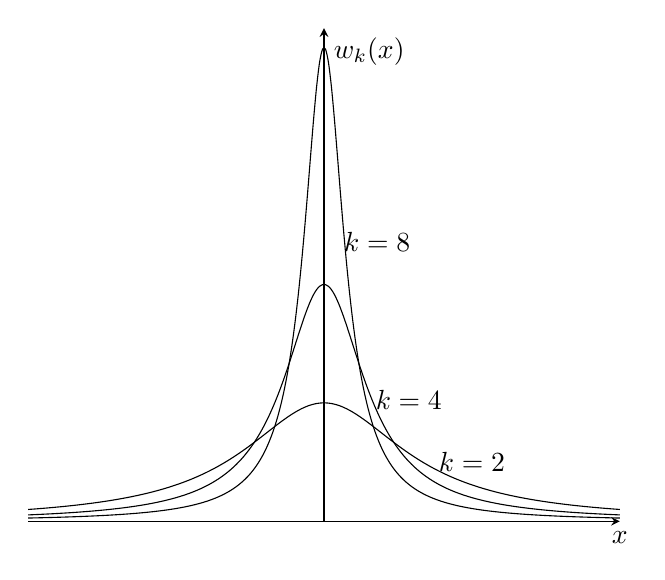
\begin{tikzpicture}
        \begin{axis}[
            axis lines = middle,
            xlabel = \(x\),
            ylabel = \(w_k(x)\),
            x label style = {anchor=north},
            xtick = {0},
            ytick= {0},
            ymin=0,
            ymax = 2.65,
            restrict y to domain=0:2.65
        ]
            \addplot[
                samples=200, 
                smooth,
                domain = -1.5:1.5
                ] 
                {2/(pi*(1+2^2*x^2))};
                \node at (axis cs:0.75, 0.32) {$k=2$};
            \addplot[
                samples=200, 
                smooth,
                domain = -1.5:1.5
                ] 
                {4/(pi*(1+4^2*x^2))};
                \node at (axis cs:0.43, 0.65) {$k=4$};
            \addplot[
                samples=200, 
                smooth,
                domain = -1.5:1.5
                ] 
                {8/(pi*(1+8^2*x^2))};
                \node at (axis cs:0.27, 1.5) {$k=8$};
        \end{axis}
    \end{tikzpicture}
    \caption{Mass Density;  eq. 3.3}
\end{figure}

If we let \(k \rightarrow \infty\), then the mass distribution approaches our idea of a point mass at \(x=0\). We would like to write
\begin{equation} \label{eq:deltaSeqLim}
    \delta(x) \overset{?}{=} \lim_{k\rightarrow \infty} w_k(x),
\end{equation}
where \(\d(x)\) is the \df{Dirac delta function}. This ``definition'' feels intuitive but is not a rigorous definition of the Dirac delta function because the limit is infinite for \(x=0\). That is, the right-hand side is not a function. We instead define the Dirac delta function, \(\d(x)\), in the following way
\begin{equation}\label{eq:seqDef}
    \begin{split}
        \lim_{k\rightarrow \inf}\intR h(x)w_k(x)dx &= \intR h(x)\d(x)dx \\
        &= h(0),
    \end{split}
\end{equation}
where \(h\) is infinitely differentiable and vanishes outside some finite interval. We call any \(w_k(x)\) which has this property a \df{\(\d\)-sequence}.  This way of defining the Dirac delta function is more rigorous while still being intuitive. However, keep in mind that the delta function is not a function. 

We would like to be able to check that a particular sequence \(w_k(x)\) is a \(\d\)-sequence. We can do this by showing that equation (\ref{eq:seqDef}) holds for \(w_k(x)\). The following theorem allows us to easily construct \(\d\)-sequences. First, we need a definition and a theorem.

% \begin{definition}
%     A function, \(f\), is \df[uniform continuity]{uniformly continuous} if for all \(\e>0\), a \(\d >0\) exists such that, if \(|a-b|<\d\), then \(|f(a)-f(b)|<\e\), for all \(a,b\in X\).
% \end{definition}

\begin{definition}
    A function, \(f: A \to \mathbb{R}\), is \df{continuous} at point \(a \in A\) for all \(\e>0\) if there exists a \(\d>0\) such that for all \(x\in A\), \(|x-y|<\d\) implies \(|f(x)-f(y)|<\e\).
\end{definition}

\begin{definition}
    A sequence of functions, \(f_k\), \df[uniform convergence]{converges uniformly} to the function, \(f(x)\), on \([a,b]\) if for any \(\e>0\) there exists an \(n\) such that \(|f_n(x)-f(x)|< \e\) for all \(x\in[a,b]\). (Note: This is a stronger notion of convergence than pointwise convergence.)
\end{definition}

\begin{theorem}
    If \(f_k(x)\) converges uniformly to \(f(x)\) on \([a,b]\), then
    \begin{equation*}
        \lim_{k\to\inf} \int_{a}^{b}f_k(x) dx = \int_{a}^{b} \lim_{k\to\inf}  f_k(x)dx = \int_{a}^{b} f(x) dx.
    \end{equation*}
\end{theorem}

\begin{theorem}\label{th:assertion}
    If \(w(x)\) is non-negative \(\intR w(x) dx = 1\), and \(w(x)=O(1/|x|^{1+\a})\) (see appendix \ref{sec:BigO} for a description of big O notation) as \(|x| \rightarrow \inf\) with \(\a>0\), then \( w_k(x) \equiv kw(kx)\) is a \(\d\)-sequence.
\end{theorem}
\begin{proof}    
    We have
    \begin{equation}\label{eq:deltaseqProof1}
        \begin{split}
            \lim_{k\rightarrow \inf}\intR w_k(x)h(x) dx &= \underbrace{\lim_{k\rightarrow\inf} \intR w_k(x)[h(x)-h(0)]dx}_I+ \underbrace{\lim_{k\rightarrow\inf} \intR w_k(x)h(0)dx}_J.
        \end{split}
    \end{equation}
    Consider \(J\),
    \begin{equation}
        \begin{split}
            J &= h(0) \lim_{k\rightarrow\inf} \intR kw(kx)dx, \ \ \text{Let  }\xi =kx\\
            &=h(0)\intR w(\xi) d\xi\\
            &= h(0).
        \end{split}
    \end{equation}
    Next, we wish to show that \(I=0\), so that the right hand side of equation (\ref{eq:deltaseqProof1}) is \(h(0)\). Let \(\epsilon > 0\), and since \(h\) is continuous at \(x=0\), there must exist a number \(\d>0\) such that \(|h(x)-h(0)|<\epsilon\) whenever \(|x-0|=|x|<\d\). Breaking up the integral \(I\),
    \begin{equation}
        \begin{split}
            I &= \underbrace{\lim_{k\rightarrow \inf} \int_{-\inf}^{-\d} w_k(x)(h(x)-h(0)) dx}_{I_1} + \underbrace{\lim_{k\rightarrow \inf} \int_{-\d}^{\d} w_k(x)(h(x)-h(0)) dx}_{I_2} \\ & + \underbrace{\lim_{k\rightarrow \inf} \int_{\d}^{\inf} w_k(x)(h(x)-h(0)) dx}_{I_3}.\\
        \end{split}
    \end{equation}
    Note that \(w_k\) converges uniformly to 0 for \(x\neq 0\) and thus, \(I_1=I_3 =0\). Since \(h\) is continuous \(|h(x)-h(0)|<\e\) whenever \(|x-0|=|x|<\d\)
    \begin{equation*}
        \begin{split}
            \left| \lim_{k\to \inf} \int_{-\d}^{\d} w_k(x)(h(x)-h(0))dx \right| & \leq  \lim_{k\to \inf} \int_{-\d}^{\d} w_k(x)|h(x)-h(0)|dx \\
            & \leq \lim_{k\to \inf} \e\int_{-\d}^{\d}w_k(x)dx\\
            &= \e \lim_{k\to \inf} \int_{-k\d}{k\d} kw(kx)dx\\
            &= \e \lim_{k\to \inf} \int_\mathbb{R} kw(kx)dx\\
            &= \e.
        \end{split}
    \end{equation*}
    Since \(\e\) may be chosen as small as we like, the integral must vanish. Thus,
    \begin{equation}
        \lim_{k\rightarrow \inf}\intR w_k(x)h(x) dx = h(0).
    \end{equation}


\end{proof}

\begin{example}
    We would like to show that the sequence
    \begin{equation*}
        w_k(x) = \begin{cases}
            k, &  0<x<\frac{1}{k}\\
            0, &x\leq 0 \text{ or } x \geq \frac{1}{k}
        \end{cases}
    \end{equation*}
    is a \(\d\)-sequence using Theorem \ref{th:assertion}. It is clear that \(w_k(x)\geq 0\)  for all \(x\) and \(w(x)=O(1/|x|^{1+\a})\) as \(|x| \rightarrow \inf\) with \(\a>0\) since it is zero when \(x \leq 0\) or \(x \geq 1/k\). Lastly, we must show that the area under \(w(x)\) is 1. Choosing \(w(x)\) so that \(kw(kx)=w_k(x)\),
    \begin{equation*}
        w(x)=\begin{cases}
            1,& 0<x<1\\
            0,& x\leq0 \text{ or } x \geq 1.
        \end{cases}
    \end{equation*}
    Clearly,
    \begin{equation}
        \begin{split}
            \intR w(x) dx &=1
        \end{split}
    \end{equation}
\end{example}

\begin{example}
    We would like to show that the sequence,
    \begin{equation}
        w_k(x) = \begin{cases}
            -k, &|x|<\frac{1}{2k}\\
            2k, &\frac{1}{2k} \leq |x| \leq \frac{1}{k}\\
            0, &|x|> \frac{1}{k},
        \end{cases}
    \end{equation}
    is a \(\d\)-sequence. Theorem \ref{th:assertion} does not apply in this case because \(w_k(x)\) is negative for some values of \(x\) so we should instead show 
    \begin{equation}
        \lim_{k\to \inf}\intR w_k(x) h(x) dx = h(0).
    \end{equation}
    To begin, we break up the integral 
    \begin{equation}
        \begin{split}
            \lim_{k\to \inf}\intR w_k(x) h(x) dx &= \lim_{k\to \inf}\int_{-\frac{1}{k}}^{-\frac{1}{2k}} 2kh(x)dx - \lim_{k\to \inf}\int_{-\frac{1}{2k}}^{\frac{1}{2k}} kh(x)dx \\
            &+ \lim_{k\to \inf}\int_{\frac{1}{2k}}^{\frac{1}{k}} 2kh(x)dx
        \end{split}
    \end{equation}
    
    Consider each integral. The mean value theorem (see Appendix A.2) shows that there exists a value, \(\x\), where \(-\frac1k < \x < -\frac{1}{2k}\), such that
    \begin{equation*}
        \begin{split}
            \lim_{k\to \inf}\int_{-\frac{1}{k}}^{-\frac{1}{2k}} 2kh(x)dx &= \lim_{k\to \inf}  \left( \left(-\frac{1}{2k} + \frac{1}{k}\right) 
            \cdot 2k\cdot h(\xi)\right) \\
            &=h(0).
        \end{split}
    \end{equation*}

    \begin{equation*}
        \begin{split}
            \lim_{k\to \inf}\int_{-\frac{1}{2k}}^{\frac{1}{2k}} -kh(x)dx &= \lim_{k\to \inf}  \left( \left(\frac{1}{2k} + \frac{1}{2k}\right) 
            \cdot -k\cdot h(\xi)\right) \\
            &=-h(0).
        \end{split}
    \end{equation*}

    \begin{equation*}
        \begin{split}
            \lim_{k\to \inf}\int_{\frac{1}{2k}}^{\frac{1}{k}} 2kh(x)dx &= \lim_{k\to \inf}  \left( \left(\frac{1}{k} - \frac{1}{2k}\right) \cdot 2k\cdot h(\xi)\right) \\
            &=h(0).
        \end{split}
    \end{equation*}
    The last step for each integral follows from the fact that as \(k \to \inf\), \(\xi\to 0\). Adding each integral shows that
    \begin{equation*}
        \lim_{k\to \inf}\intR w_k(x) h(x) dx = h(0).
    \end{equation*}
\end{example}

\subsection{The Dirac Delta Function as a Generalized Function}
The Dirac delta function can also be defined as a generalized function. To understand this, we will begin by defining some terms.

\begin{definition}
     A \df{closed region} is one that includes its boundary.
\end{definition}

\begin{definition}
    The \df{support} of a function, \(f\), is the subset, \(\mathcal{S}\), of the domain of \(f\) where \(f\) is nonzero.
\end{definition}

\begin{definition}
    A function has \df{compact support} if its support is closed and bounded.
\end{definition}
We will denote the space of infinitely differentiable functions with compact support by \(\mathcal{D}\).

\begin{definition}
    A \df{continuous functional} is a functional \(\mathcal{F}\) on \(\mathcal{D}\), is a continuous functional if for any functional sequence \(g_k\) in \(\mathcal{D}\) which converges to \(g\) in \(\mathcal{D}\) as \(k \to \infty\), then the numerical sequence \(F(g_k)\) converges to \(F(g)\).
\end{definition}

\begin{definition}
    \df[generalized function]{Generalized functions} are linear functionals that are continuous on \(\mathcal{D}\).
\end{definition}

We consider the following functional,
\begin{equation}\label{eq:generalizedFunction}
    \mathcal{F}(h) = \int_{-\infty}^{\infty} g(x)h(x)dx,
\end{equation}
where \(g\) is some fixed integrable function. This functional assigns a numerical value, \(\mathcal{F}(h)\), for each function \(h\) within the domain, \(\mathcal{D}\), of \(\mathcal{F}\).

\begin{example}
    Suppose \(\mathcal{F}(h)\) is the integral of \(h\) from \(\xi\) to \(\infty\),
    \begin{equation}
        \int_{\infty}^{\infty} g(x)h(x)dx = \int_{\xi}^{\infty} h(x) dx.
    \end{equation}
    Then, \(g(x)\) is equivalent to the \df{Heaviside step function},
    \begin{equation}
        H(x) = \begin{cases}
            1, & x>0\\
            0, & x<0\\
            \frac{1}{2}, & x=0,
        \end{cases}
    \end{equation}
    which is a function in the classical sense. \footnote{We have defined \(H(0)\) to be \(\frac{1}{2}\), which is a common convention. However, for our purposes, the value at any particular point is not important since we are only ever interested in integrating the function.}    
\end{example}

If \(\mathcal{F}(h)\) is \(h(0)\) so that
\begin{equation}\label{eq:introtodelta}
    \int_{-\infty}^{\infty}g(x)h(x) dx=h(0)
\end{equation}
then it can be shown that there is no function, \(g(x)\), which exists such that equation (\ref{eq:introtodelta}) is true for all functions, \(h(x)\), in the domain, \(\mathcal{D}\). We call \(g\) defined by equation (\ref{eq:introtodelta}) a generalized function, and in particular, it is the Dirac delta function. As such, \(\delta\) is defined in the following way,
\begin{equation}\label{eq:deltadef}
    \int_{-\infty}^{\infty} \delta(x)h(x) dx = h(0)
\end{equation}
for all \(h\in \mathcal{D}\).

Although \(\delta(x)\) has support only at \(x=0\), it can be adjusted to have support at any point by shifting the argument. Thus, \(\delta(x-\xi)\) acts at \(x=\xi\), \footnote{By saying that \(\d\) acts at \(x=\x\), we mean that \(\d(x-\x)\) has support only at \(x=\x\) and 
\begin{equation*}
    \int_{-\infty}^{\infty} \delta(x - \x )h(x) dx = h(\xi).
\end{equation*} }
\begin{equation}
    \int_{-\inf}^{\infty} \delta(x-\xi)h(x)dx = h(\xi).
\end{equation}

\begin{definition}
    We define the derivative of a generalized function by integrating by parts
    \begin{equation}
            \intR g'(x)h(x) dx= g(x)h(x)\biggr\rvert_{-\infty}^{\infty} - \intR g(x)h'(x)dx.
    \end{equation}
\end{definition}
The integral term is fairly simple to interpret since it is of the same form as equation (\ref{eq:generalizedFunction}), but the boundary term is not as nice because it involves knowing the values of \(g\), which are never known. However, our restriction that \(h\) has compact support gives the intuition that it must vanish at infinity, and since we are integrating from \(-\inf\) to \(\inf\), we define the boundary term to be zero. We define
\begin{equation}
    \intR g'(x)h(x)dx = -\intR g(x)h'(x)dx.
\end{equation}
For the Dirac delta function, this means
\begin{equation}
    \begin{split} \label{eq:deltafirst}
        \intR \delta'(x-\xi)h(x)dx &= -\intR\delta(x-\xi)h'(x)dx\\
        &=-h'(\xi).
    \end{split}
\end{equation}


\begin{theorem} \label{th:deltad}
    The \(j\)th derivative of the Dirac delta function is defined by
    \begin{equation}
         \intR \delta^{(j)}(\xi-x)h(\xi)d\xi = (-1)^jh^{(j)}(x).
    \end{equation}
\end{theorem}
\begin{proof} We prove the statement by induction.\\
    \textbf{Base step:} Proven to be true for \(k\) = 1 in equation (\ref{eq:deltafirst}).\\
    \textbf{Induction step:} Let \(k \in \mathbb{N}\) and suppose the statements holds for some \(k\geq 1\). Then,
    \begin{align*}
        \intR \delta^{(k+1)}(\xi-x)h(\xi)d\xi &= \d^{(k)}(\xi-x)h(\xi)\bounds{-\inf}{\inf}-\intR \delta^{(k)}(\xi-x)h'(\xi)d\xi\\
        &=-\intR \delta^{(k)}(\xi-x)h'(\xi)d\xi\\
        &=-(-1)^{k}(h')^{(k)}(x)\\
        &=(-1)^{k+1}h^{(k+1)}(x).
    \end{align*}
\end{proof}

Note that because of the discontinuity in \(H(x-\xi)\) at the point \(x=\xi\), the derivative of \(H\) does not exist as an ordinary function. However, the previous method does allow us to find \(H'(x-\xi)\) as a generalized function, 
\begin{equation}
    \begin{split}
        \intR H'(x-\xi)h(x)dx &= -\intR H(x-\xi)h'(x)dx\\
        &=-\int_{\xi}^{\infty}h'(x)dx \\
        &= h(\xi).
    \end{split}
\end{equation}
Since
\begin{equation}
    \intR \delta(x-\xi)h(x)dx=h(\xi)
\end{equation}
it must be the case that, in the sense of generalized functions,
\begin{equation}\label{eq:Hprime}
    H'(x-\xi) = \delta(x-\xi).
\end{equation}
Such equalities between generalized functions, as seen in (\ref{eq:Hprime}), are understood in the sense that if some \(h\) in \(\mathcal{D}\) is multiplied through, and we integrate over \((-\infty, \infty)\) then the result will hold. To wit, we consider generalized functions, \(g_1\) and \(g_2\), to be equal if, for all \(h\in \mathcal{D}\),
\begin{equation}
    \intR g_1(x)h(x)dx = \intR g_2(x)h(x)dx.
\end{equation}

Notice that for all \(n > 0\)
\begin{equation}
    x^n\delta(x)=0
\end{equation}
as a result of
\begin{equation}
    \intR x^n\delta(x)h(x)dx=[x^nh(x)]|_{x=0} = 0.
\end{equation}

\begin{example}
    We would like to show that \(e^x\d(x)=\d(x)\). To begin with, we integrate \(e^x\d(x)f(x)\) and would like to show that this is equal to \(f(0)\) to satisfy the generalized function definition of the delta function. We have
    \begin{equation}
        \begin{split}
            \intR e^x\d(x)f(x)dx &= \intR \d(x)\underbrace{e^xf(x)}_{g(x)}dx\\
            &=\intR \d(x)g(x)dx\\
            &=g(0)\\
            &=e^0f(0)\\
            &=f(0).\\
        \end{split}
    \end{equation}
    Therefore
    \begin{equation}
        \intR e^x\d(x)f(x)dx = \intR \d(x)f(x)dx
    \end{equation}
\end{example}
\begin{example}
    We would like to show that \(\frac{d^4}{dx^4}|x|^4 = 12\d(x)\). Note that \(|x|=2xH(x)-x\). We begin by manipulating \(|x|^3\) into a more convenient form.
    \begin{equation}
        \begin{split}
            |x|^3 &= (2xH(x)-x)^3\\
            &=x^3(2H(x)-1)^3\\
        \end{split}
    \end{equation}
    Next, it is useful to simplify. Note that \(H^n(x)=H(x)\), \(n\in\mathbb{N}\). We find
    \begin{equation}
        \begin{split}
            (2H(x)-1)^3 &= (2H(x))^3-3(2H(x))^2+3(2H(x))-1\\
            &=8H(x)-12H(x)+6H(x)-1\\
            &=2H(x)-1.
        \end{split}
    \end{equation}
    Finally, we find the fourth derivative,
    \begin{equation}
        \begin{split}
            D^4(x^3(2H(x)-1)) &= D^3(3x^2(2H(x)-1) +2x^3\d(x))\\
            &=D^3(3x^2(2H(x)-1))\\
            &= D^2(6x(2H(x)-1) + 6x^2\d(x))\\
            &=D^2(6x(2H(x)-1))\\
            &= D(12(H(x)-1) + 12x\d(x))\\
            &= D(12(H(x)-1))\\
            &= 12\d(x).
        \end{split}
    \end{equation}
\end{example}

\section{The Method of Green's Functions}
\setcounter{example}{0}
\subsection{Introduction}
    A \df{Green's function} is the solution to a differential equation of the form
    \begin{equation} \label{eq:greensdef}
        \opp{L^*_\xi} G(\xi, x) = \delta(\xi - x)
    \end{equation}
    satisfying boundary conditions related to those applied to the function of interest.
    The subscript \(\xi\) on the differential operator indicates that the derivatives are being taken with respect to the variable \(\xi\). By making use of some of the delta function's unusual properties, Green's functions can be used to solve nonhomogeneous linear differential equations.

    To find the solution to the linear differential equation
    \begin{equation} \label{eq:4.2}
        \opp{L}u=\phi,
    \end{equation}
    we start by finding the formal adjoint as in equation (\ref{eq:adjoint}). If we replace \(v\) with \(G\), and we replace \(x\) with a dummy variable \(\xi\), we are left with an equation of the form
    \begin{equation} \label{eq:greenadjoint}
        \intl G(\xi, x)\opp{L}u(\xi) d\xi = \bterms + \intl u(\xi)\opp{L^*}G(\xi,x) d\xi.
    \end{equation} 
    It follows from equation (\ref{eq:greensdef}) that we can replace \(\opp{L^*}G\) with \(\d\), and from equation (\ref{eq:4.2}) that we can replace \(\opp{L}u\) with \(\phi\), 
    \begin{equation}
        \begin{split}
            \intl G(\xi,x)\phi(\xi) d\xi &= \bterms + \intl u(\xi)\d(\xi-x) d\xi\\
            &=\bterms + u(x).
        \end{split}
    \end{equation}
    Therefore, if we choose boundary conditions for \(G\) such that the boundary terms do not depend on \(u\) and we are able to find \(G\), then finding \(u\) is reduced to a problem of integrating \(G\phi\). 

    To illustrate the key ideas of the method, we will consider several examples which begin simply and become more complex. Each example will be concerned with a key concept in implementing the method of Green's functions.

\subsection{Example 1 \textit{Loaded String}}
    
    Consider the boundary value problem
    \begin{equation} \label{ex1:initialize}
        u''(x) = \phi(x);\quad u(0)=u(1)=0
    \end{equation}
    where \(\phi(x)\) is prescribed. Equation (\ref{ex1:initialize}) can be regarded as describing the static deflection of a string under unit tension between fixed endpoints and subjected to a force distribution \(\phi(x)\).

    To show that this differential equation does describe the loaded string, we first assume \(|u(x)|<<1\). Then, consider a local area of the deflected string which has tension, \(\bf{T_1}\), in one direction and tension, \(T_2\), in the other, and a small amount of mass downward (Figure 4.1). We draw a free-body diagram for this in Figure 4.2. We can see that via Newton's second law of motion,
    \begin{equation*}
        \begin{split}
            \Sigma \mathbf{F} &= m\opp{a}\\
            \opp{T_1} + \opp{T_2} + dm\opp{g} = 0
        \end{split}
    \end{equation*}
    In the \(x\) direction that is,
    \begin{equation}\label{eq:xdir}
        -T_1\cos \theta_1 + T_2 \cos\theta_2 = 0,
    \end{equation}
    and in the \(y\) direction
    \begin{equation}\label{eq:ydir}
        -T_1\sin\theta_1 + T_2\sin\theta_2 = dm\opp{g}.
    \end{equation}
    Because the deflection of the string is small, \(\theta_1\) and \(\theta_2\) must be much less than 1, and so by the small angle approximation,
    \begin{equation*}
        \cos \theta_1 \approx \cos \theta_2 \approx 1,
    \end{equation*}
    and therefore, from equation (\ref{eq:xdir}), \(T_1=T_2=T\). Also, by the small angle approximation \(\tan \theta\approx u'(x)\). Additionally, \(dmg = \rho g ds\) where \(ds\) is a small element of arc length, so 
    \begin{equation*}
        \begin{split}
            ds &= \sqrt{(dx)^2 + (u')^2dx}\\
            &\approx dx.
        \end{split}
    \end{equation*}
    
    Applying this to equation (\ref{eq:ydir}), we see that 
    \begin{equation*}
        \begin{split}
            T(\tan\theta_2-\tan\theta_1) &\approx \phi ds\\
            T(u'(x_2)-u'(x_1)) & \approx \phi dx\\
            \frac{u'(x_2)-u'(x_1)}{dx} &\approx \frac{\phi}{T},\quad \text{Let } T=1\\
            u''(x)&\approx \phi(x).
        \end{split}
    \end{equation*}
    \begin{figure}
        \centering
        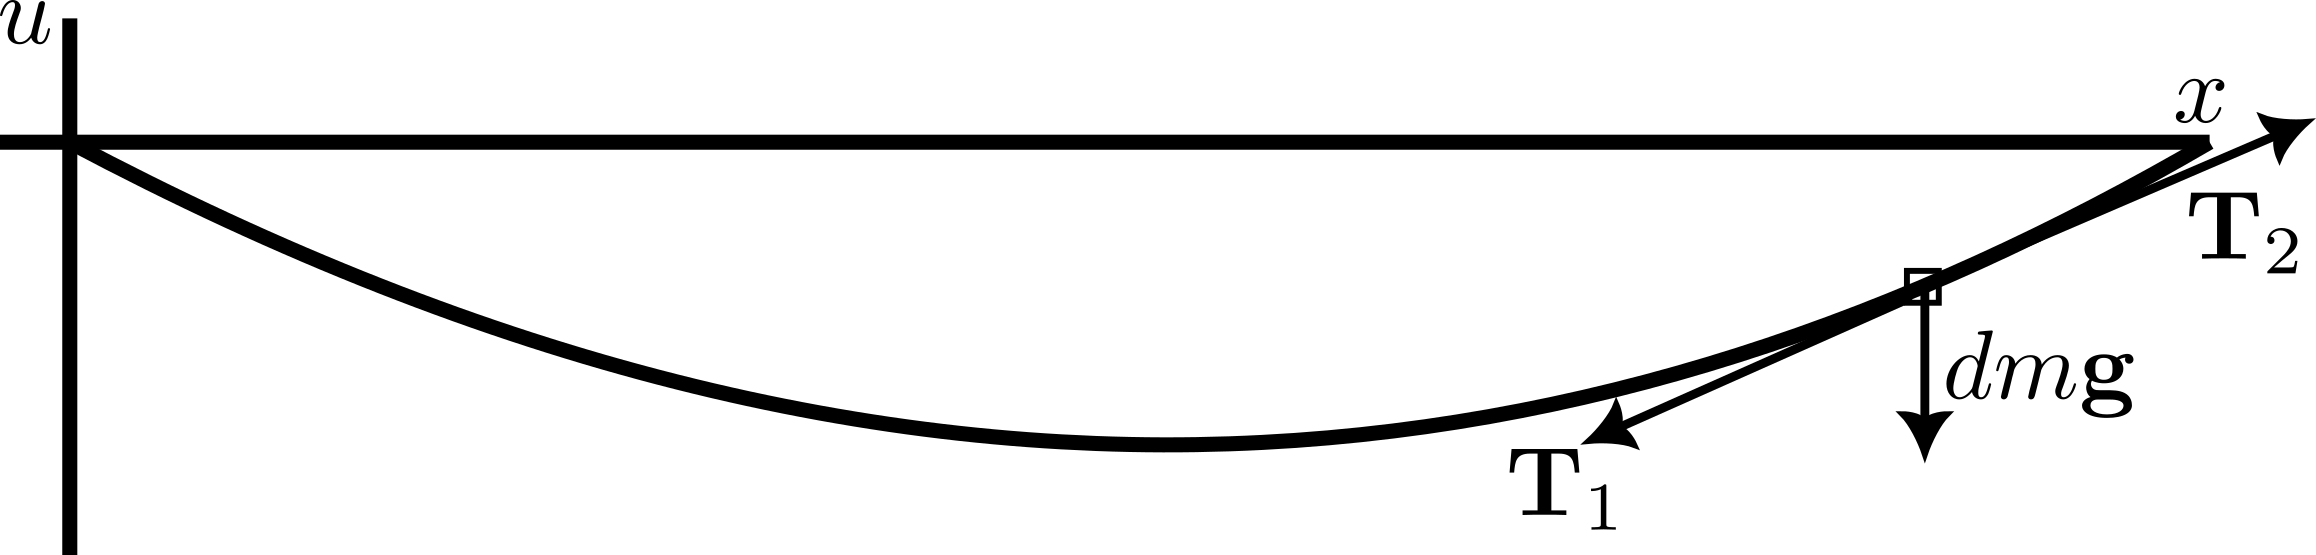
\includegraphics[width=0.6\linewidth]{include/loadtension1.png}
        \caption{Loaded string with tensions.}
    \end{figure}

    \begin{figure}
        \centering
        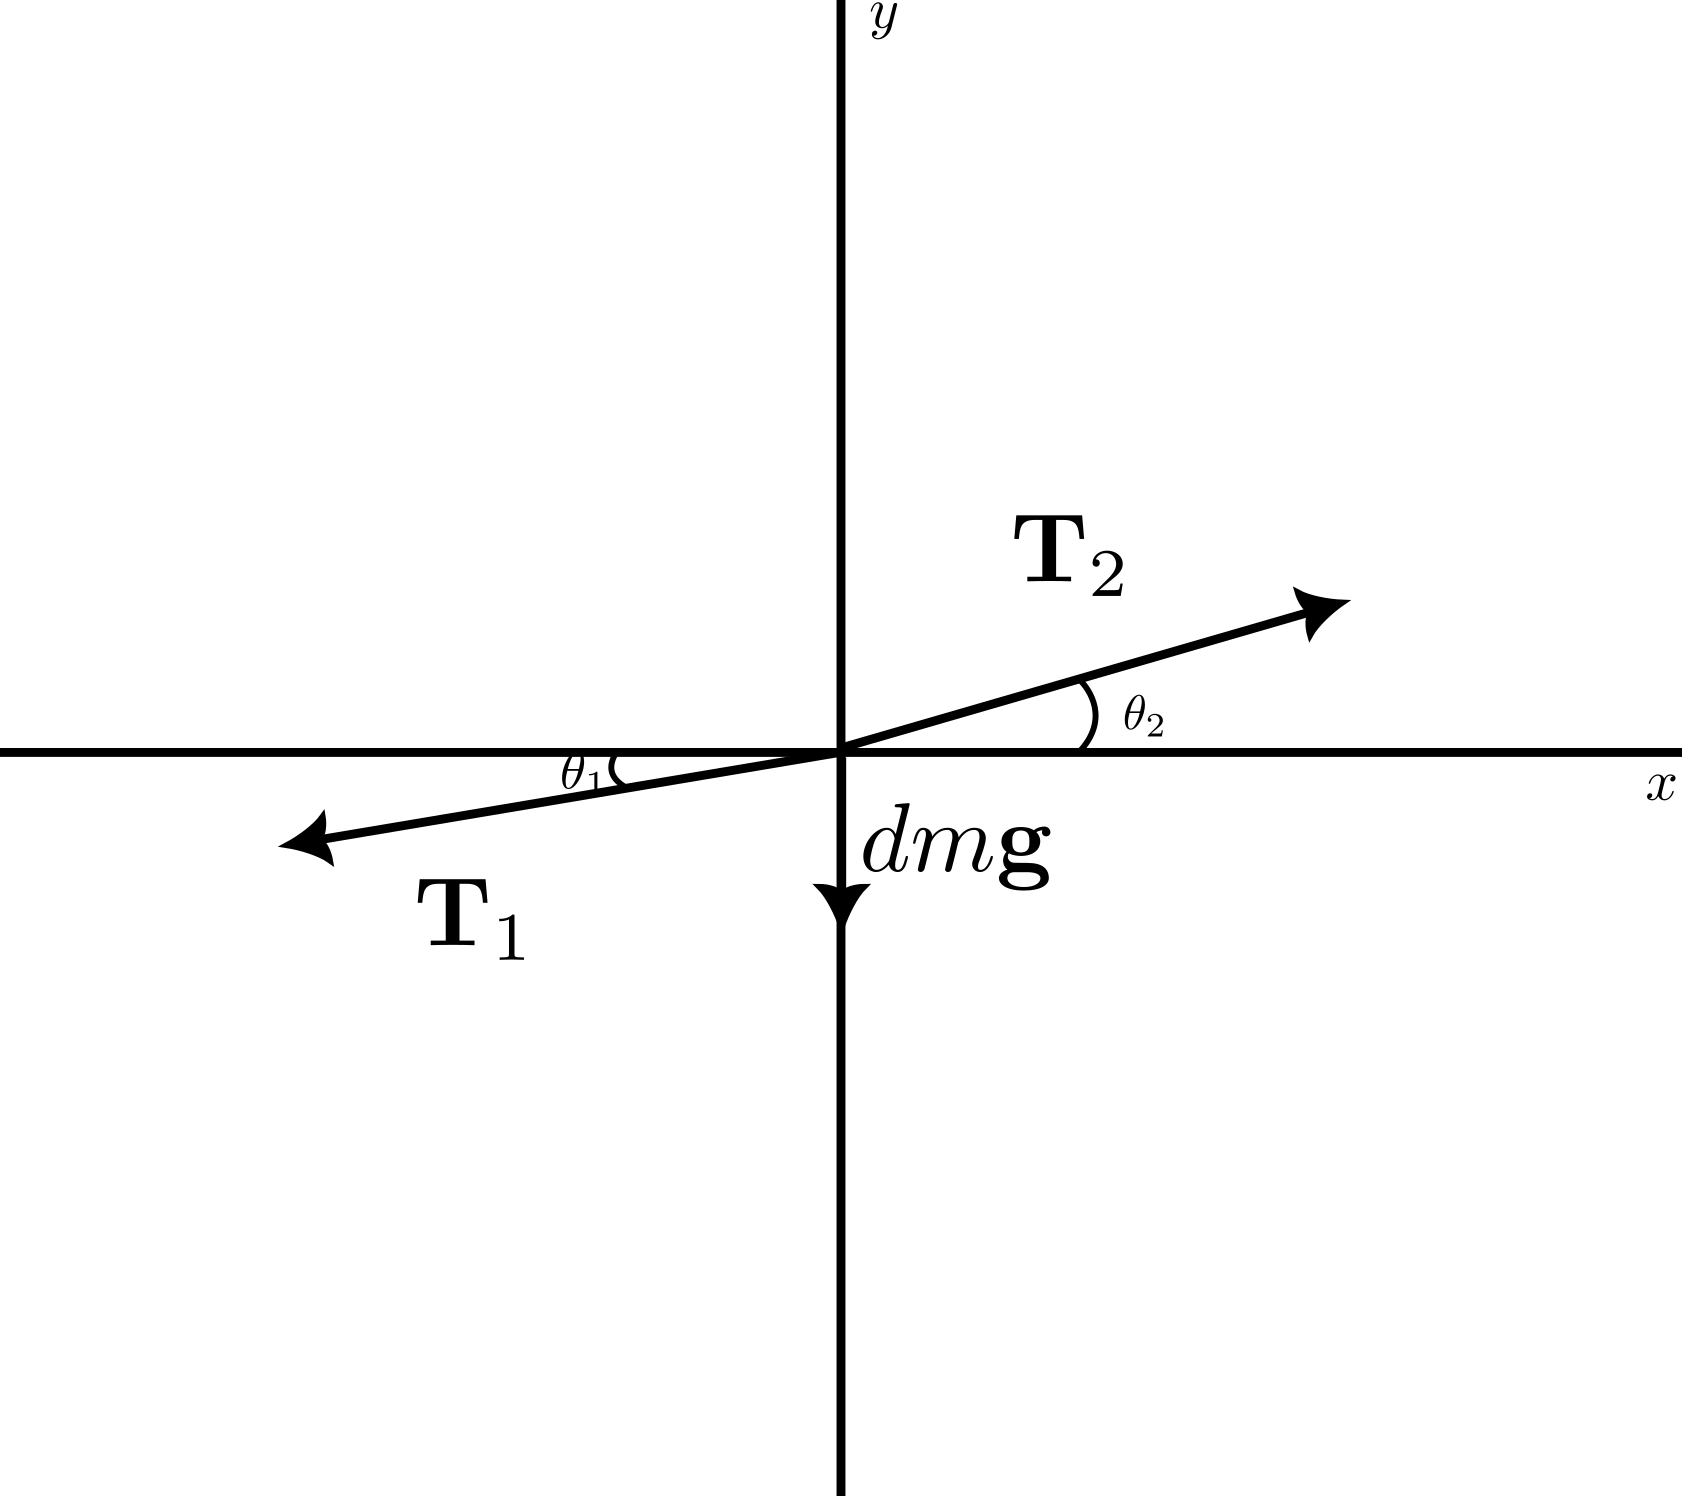
\includegraphics[width=0.6\linewidth]{include/loadtension2.png}
        \caption{Loaded string free-body diagram.}
    \end{figure}

    \begin{figure}\label{fig:LoadedString}
    \centering
    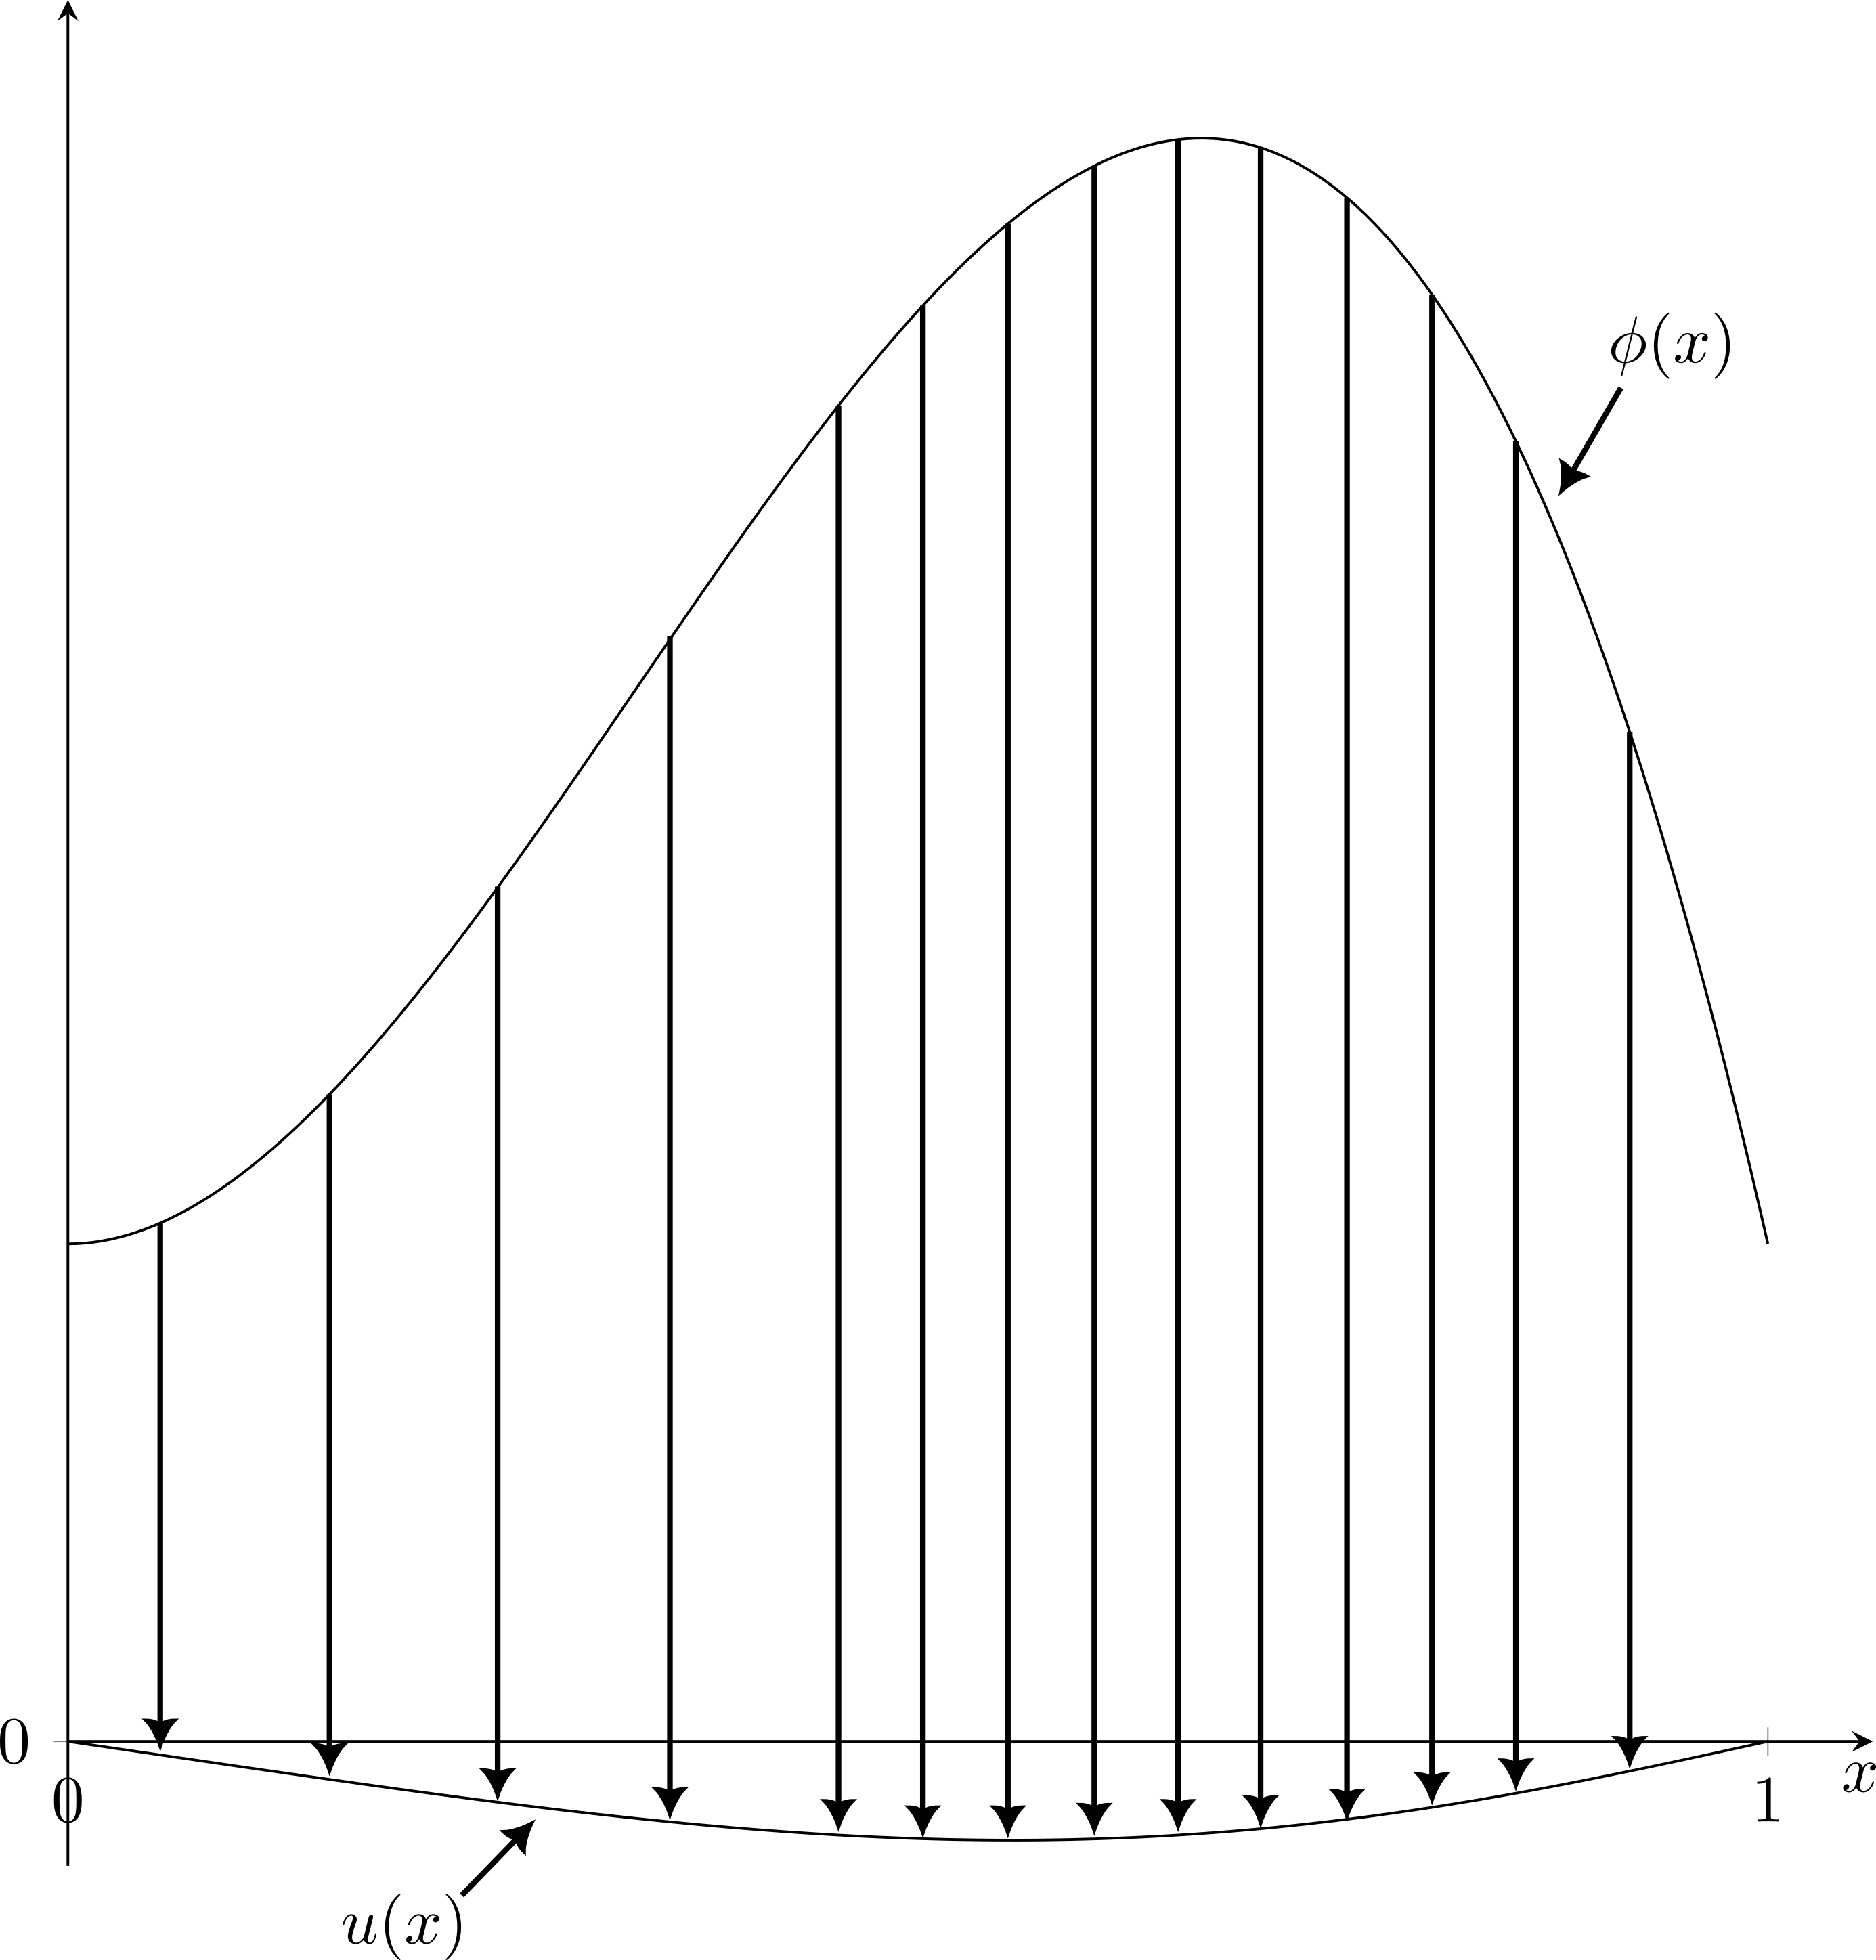
\includegraphics[width=0.5\linewidth]{include/loadedstring.png}
    \caption{Loaded String}
\end{figure}
    
    To find a solution to this differential equation, we first find the formal adjoint \(\Lstar\) as in equation~(\ref{eq:greenadjoint}), 
    \begin{equation}
        \begin{split}
            \int_{0}^{1} G(\xi, x)\L u(\xi) d\xi  &= (G(\xi, x)u'(\xi)-G_\xi (\xi, x)u(\xi))\biggr\rvert_0^1 + \int_{0}^{1} uG_{\xi\xi}d\xi\\
            &= G(1, x)u'(1) - G_\xi(1, x)u(1) \\&- G(0, x)u'(0) + G_\xi(0,x)u(0) + \int_{0}^{1} uG_{\xi\xi}d\xi.
        \end{split}
    \end{equation}
    Therefore, 
    \begin{equation}
        \Lstar = \frac{d^2}{d\xi^2}
    \end{equation}
    and 
    \begin{equation}\label{eq:loadedStringLstarG}
        \Lstar G = G_{\xi\xi} = \delta(\xi-x).
    \end{equation}
    Because of the boundary conditions on \(u\) in equation (\ref{ex1:initialize}), two of our boundary terms are zero. Thus,
    \begin{equation}
        \int_{0}^{1} G(\xi, x)\L u(\xi) d\xi = G(1, x)u'(1) - G(0, x)u'(0) + \int_{0}^{1} uG_{\xi\xi}d\xi.
    \end{equation}
    Now, we want to remove the \(u\) dependency from the boundary terms and, as such, impose the conditions that
    \begin{equation}\label{eq:LoadedstringGBounds}
        G(1,x) = G(0,x) = 0.
    \end{equation}
    Then, provided we can find \(G\) satisfying equations (\ref{eq:loadedStringLstarG}) and (\ref{eq:LoadedstringGBounds}),the solution is given by 
    \begin{equation}\label{eq:loadSln}
        u(x) = \int_0^1 G(\xi,x)\phi(\xi)d\xi.
    \end{equation}
    To find the Green's function, we integrate equation (\ref{eq:loadedStringLstarG}), regarding \(x\) as fixed.
    \begin{equation}
        \begin{split}
            G_\xi &= H(\xi-x) + A(x)\\
            G &= (\xi - x)H(\xi-x)+A(x)\xi +B(x)
        \end{split}
    \end{equation}
    Imposing the boundary conditions, 
    \begin{equation}
        \begin{split}
            &G(0,x) = 0 = B(x)\\
            &G(1,x) = 0 =  1 - x + A(x) + B(x),
        \end{split}
    \end{equation}
    shows us that \(B(x)=0\) and  \(A(x)=x-1\). Therefore
    \begin{equation}\label{eq:LoadGf}
        G(\xi,x) = (\xi-x)H(\xi-x) + (x-1)\xi.
    \end{equation}

    Equation (\ref{eq:loadedStringLstarG}) can, like equation (\ref{ex1:initialize}), be interpreted as the deflection of a loaded string. Specifically, it is the deflection as a function of \(\xi\) due to a point load of unit strength at \(x=\x\), \(\d(\xi-x)\), instead of a load distribution, \(\phi\). Rewriting our Green's function as
    \begin{equation}
        G(\xi,x)= \begin{cases}
            (x-1)\xi, & \xi \leq x\\
            (\xi-1)x, & > \geq x
        \end{cases}
    \end{equation}
    makes it clear that \(G(\xi,x)\) is symetric, to wit: \(G(\xi,x)=G(x,\xi)\). This is often referred to as ``Maxwell Reciprocity.'' Because of this reciprocity, \(G(\xi,x)\) is also the deflection, as a function of \(x\), due to a unit load at \(\xi\). Then, \(G(\xi,x)\phi(\xi)d\xi\) is the deflection due to an incremental load \(\phi(\xi)d\xi\) at \(\xi\). As such, equation (\ref{eq:loadSln}) represents the superposition of these deflections. It is important to recognize that the superposition nature of equation (\ref{eq:loadSln}) is a result of the linearity of \(\mathcal{L}\).

    Additionally, it should be noted that the boundary terms do not always vanish. For example, if we change the boundary condition \(u(1)=0\) to \(u(1)=\a\), then
    \begin{equation*}
        u(x)=\a x + \int_{0}^{1} G(\xi,x)\phi(\xi)d\xi.
    \end{equation*}
    Here, \(G\) is still given by equation (\ref{eq:LoadGf}) because changing the boundary conditions on \(u\) in this way, does not change that the boundary conditions on \(G\) need to be such that 
    \begin{equation*}
        G(0,x)u'(0) = 0 \text{ and } G(1,x)u'(1)=0.
    \end{equation*}

    \subsection{Example 2 \textit{Infinite Beam on an Elastic Foundation}}
    It is prudent to, next, consider a differential operator defined over an infinite interval. We imagine an infinitely long beam on an elastic foundation. According to the classical Euler beam theory, the deflection, \(u(x)\), resulting from a net loading, \(p(x)\) force per unit length, satisfies the differential equation
    \begin{equation*}\label{eq:loadedStringStart}
        (EIu'')'' = p(x).
    \end{equation*}
    \begin{figure}
        \centering
        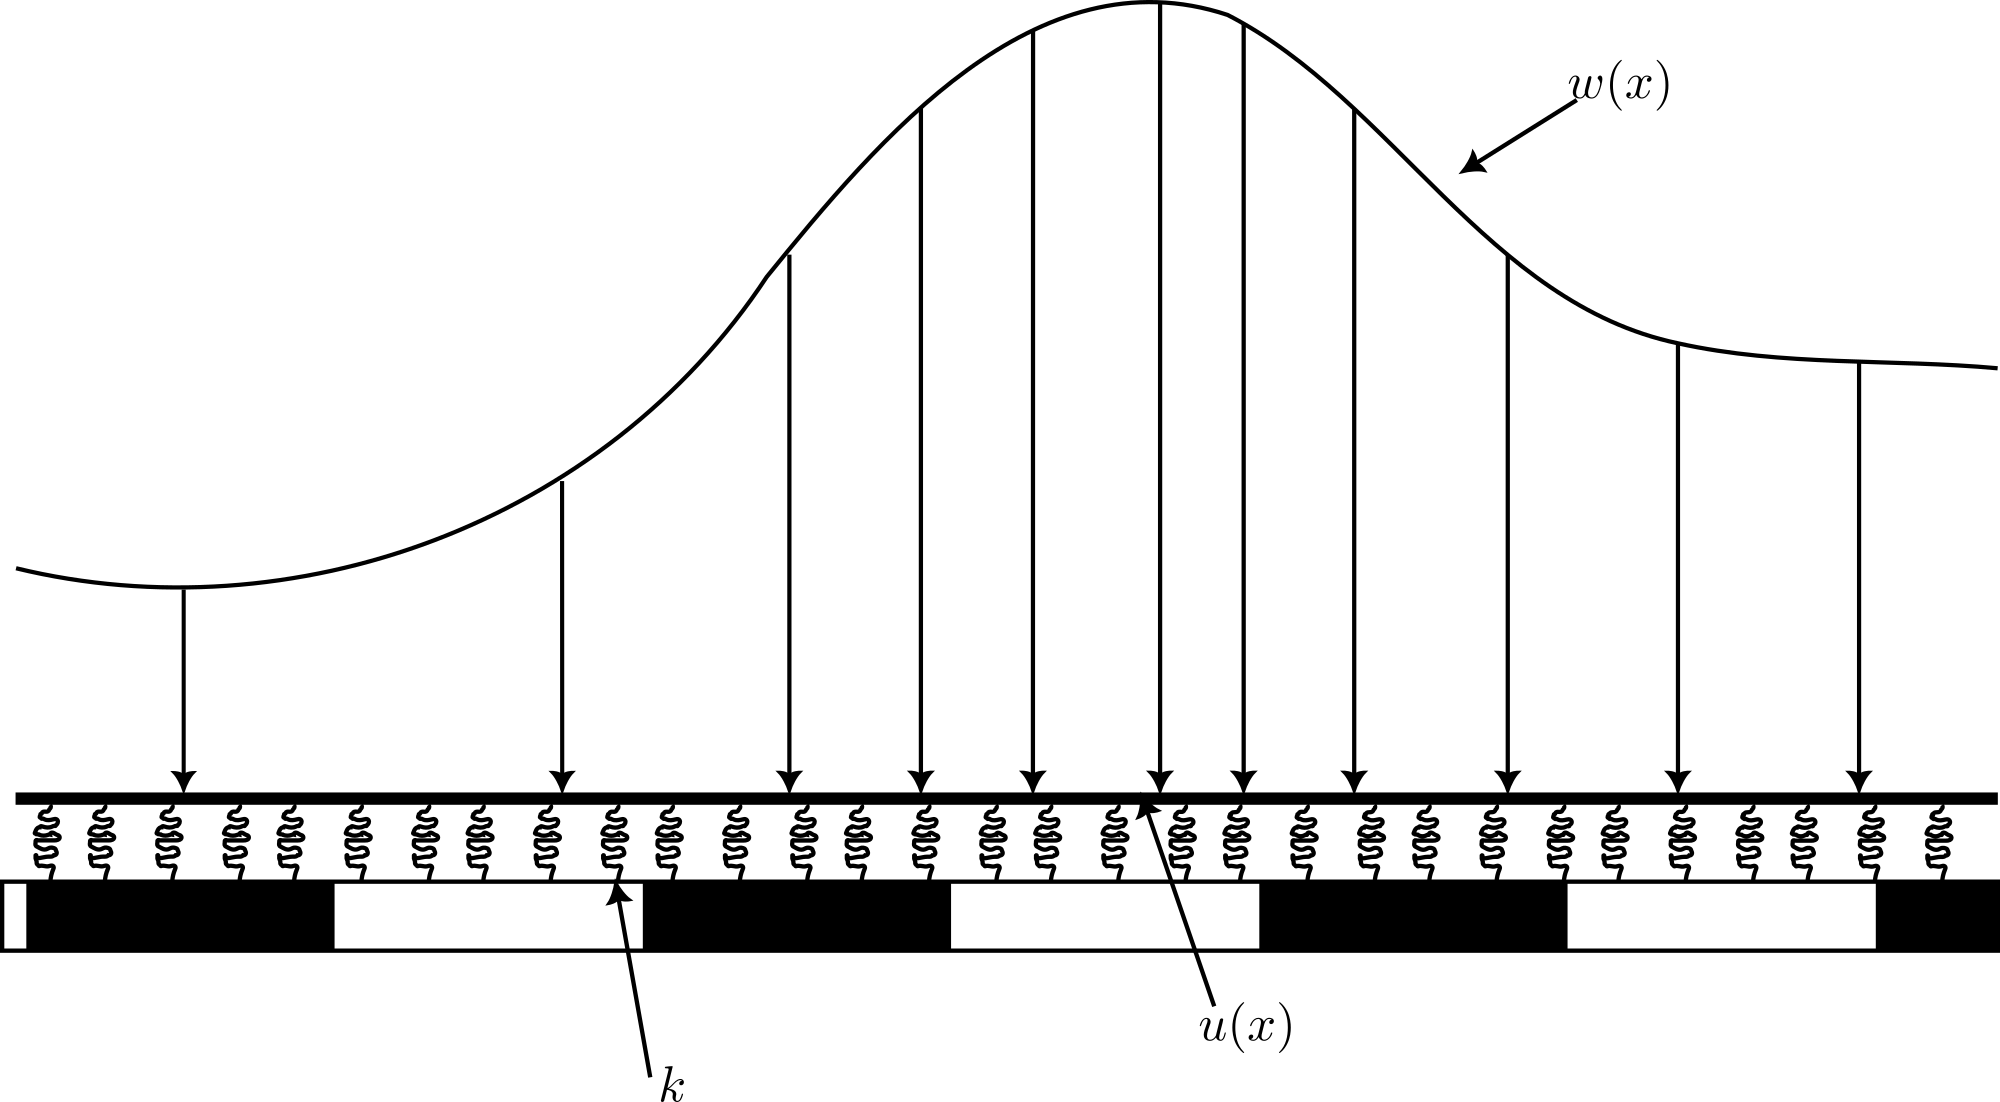
\includegraphics[width=0.75\linewidth]{include/Beam.png}
        \caption{Infinite beam on elastic foundation}
    \end{figure}

    Where the flexural rigidity of the beam, \(EI\), may be a function of \(x\). We also consider the spring constant per unit length,\(k\). For the purposes of this example, we consider both \(EI\) and \(k\) to be constant and the prescribed loading to be \(w(x)\), where \(p(x) = w(x)-ku(x)\). By substituting these into equation (\ref{eq:loadedStringStart}) it becomes
    \begin{equation*}
        EIu^{(4)}(x)+ku(x)=w(x).
    \end{equation*} 
    or
    \begin{equation*}
        u^{(4)}(x) + \a^4u(x)= W(x)
    \end{equation*}
    where
    \begin{equation*}
        \a =\frac{k}{EI} \text{ and } W(x)= \frac{w(x)}{EI}.
    \end{equation*}
    For boundary conditions, we only require that \(W(x)\) be such that \(u\) and each of its first three derivatives approach a finite value as \(|x|\to \inf\).

    As before, we integrate by parts:
    \begin{equation*}
        \intR G\L u d\x = (Gu'''-G_\x u'' + G_{\x\x}u' - G_{\x\x\x}u)\bounds{-\inf}{\inf} + \intR u\Lstar Gd\x.
    \end{equation*}
    where \(\Lstar = \L\). 

    Then, 
    \begin{equation}\label{eq:LGDeltaBeam}
        \L G = G_{\x\x\x\x} + \a^4 G = \d(\x-x).
    \end{equation}
    When \(\x \neq x\)
    \begin{equation*}
        G_{\x\x\x\x} + \a^4 G = 0.
    \end{equation*}
    By substituting \(G=e^{m\x}\) we find the auxiliary equation \(m^4+m=0\), so
    \begin{equation*}
        \begin{split}
            m^4 &= -\a^4\\
            m^4 &= \a^4e^{i\pi(2n+1)}\\
            m&= \a e^{i\pi(2n+1)/4}\\
            &= \a \{e^{i\pi/4}, e^{i3\pi/4}, e^{i5\pi/4}, e^{i7\pi/4}\}
        \end{split}
    \end{equation*}
    Thus, for \(\x\neq x\), \(G\) is of the form
    \begin{equation*}
        \begin{split}
            e^{m\x} &= ce^{\a (\pm \frac{1}{\sqrt{2}} \pm \frac{1}{\sqrt{2}}i)\x}\\
            &= (ae^{\a\x/\sqrt{2}}+be^{-\a\x/\sqrt{2}})  (c\cos(\a\x/\sqrt2) + d\sin(\a\x/\sqrt2))
        \end{split}
    \end{equation*}
    with  different values for \(a,b,c,d\) to either side of \(x\). By applying the boundary, continuity, and jump conditions, one can show that 
    \begin{equation*}
        G(\x,x) = \frac{e^{-\a|\x-x|/\sqrt2}}{2\a^3}\sin(\frac{\a|\x-x|}{\sqrt2}+ \frac\pi4).
    \end{equation*}
    This result can also be found by Fourier and complex analysis which is beyond the scope of this paper.
\subsection{Sturm-Liouville Equations}
    We are interested in finding the Green's function for the general second-order linear differential operator
    \begin{equation}
        \L = \D(p\D)+q
    \end{equation}
    with the general unmixed boundary conditions
    \begin{equation*}
        \opp{B}_1(u) =\a_{1}u(\lima)+\a_{2}u'(\lima) = 0,\quad \opp{B}_2(u) = \b_{1}u(\limb)+\b_{2}u'(\limb) = 0
    \end{equation*}
    where \(p\) and \(q\) are functions of the independent variable. Differential operators of this form are \df{Sturm-Liouville differential operators}. By referring to equation (\ref{eq:2OAdjoint}), it is clear that Sturm-Liouville differential operators are self-adjoint since \(a=p\) and \(b=p'\). 

    To analyze these equations, we define the conjunct. Recall from equation (\ref{eq:2OAdjoint}) that for a second-order differential operator, which is not necessarily self-adjoint,
    \begin{equation*}
        \Lstar v = av''+(2a'-b)v'+(a''-b'+c).
    \end{equation*}
    It follows that 
    \begin{equation*}
        \intl (v\L u - u\Lstar v)dx = J(v,u)\bounds{\lima}{\limb},
    \end{equation*}
    where
    \begin{equation*}
        \begin{split}
            J(v,u) &= avu'-a'vu-av'u + bvu\\
            &=avu'- u(av)' +bvu
        \end{split}
    \end{equation*}
    is the \df{conjunct} of \(v\) and \(u\).

    We now return to our Sturm-Liouville differential operator, \(\L\), with boundary conditions \(\opp{B}_1(u)=\opp{B}_2(u)=0\). We also assume that \(p(x)\neq 0\) on the interval \(\lima \leq x\leq \limb\). 

    The Green's function \(G(\xi,x)\), is the solution to the equation
    \begin{equation}\label{eq:SLGDE}
        \L_\xi G = (p(\xi)G_\xi(\xi,x))_\xi-q(\xi)G(\xi,x)=\d(\xi-x),
    \end{equation}
    which satisfies the boundary conditions \(\opp{B}_1(G)=\opp{B}_2(G)=0\). Such an equation has two linearly independent solutions, \(v_1(\xi)\) and \(v_2(\xi)\). Now to account for the boundary conditions we let \(w_1(\xi)\) be a linear combination of \(v_1(\xi)\) and \(v_2(\xi)\) which satisfies \(\df{B}_1(w_1(x)) = 0\) and let \(w_2(x)\) be a linear combination of \(v_1(\xi)\) and \(v_2(\xi)\) which satisfies \(\df{B}_2(w_2(x)) = 0\). Preliminarily our Green's function is of the form
    \begin{equation*}
        G(\xi,x)=\begin{cases}
            a_1(x)w_1(\xi), & \xi < x\\
            a_2(x)w_2(\xi), & \xi > x.
        \end{cases}
    \end{equation*}
    This satisfies the boundary conditions because we defined it as such and satisfies equation (\ref{eq:SLGDE}) everywhere except at \(\x=x\). However, we see that \(G_\x(\xi, x)\) has a discontinuity at \(\xi=x\), and \(G\) is continuous. For \(G\) to be continuous, it must satisfy
    \begin{equation*}
        G(x^+, x) = G(x^-, x).\footnote{Here, \(x^+\) and \(x^-\) are shorthand for \(\x\) as approached from the right or left side respectively. That is to say %TODO Check footnote
        \begin{equation*}
            G(x^+, x) = \lim_{\e\to 0^+} G(x+\e, x)
        \end{equation*}
        and
        \begin{equation*}
            G(x^-, x) = \lim_{\e\to 0^+} G(x-\e, x)
        \end{equation*}}
    \end{equation*}
    Therefore, 
    \begin{equation*}
        a_1(x)w_1(x) = a_2(x)w_2(x)
    \end{equation*}
    and so
    \begin{equation*}
        a_1(x)=c(x)w_2(x), \quad a_2(x)=c(x)w_1(x).
    \end{equation*}
    Substituting into \(G\) results in
    \begin{equation*}
        G(\xi,x)=\begin{cases}
            c(x)w_1(\xi)w_2(x), &\xi < x\\
            c(x)w_1(x)w_2(\xi), &\xi > x.
        \end{cases}
    \end{equation*}
    Next, we must find the jump condition by integrating as follows:
    \begin{equation*}
        \begin{split}
            \int_{x^-}^{x^+} L_\xi G(\x,x) d\x &= \int_{x^-}^{x^+} \d(\x-x)d\x = 1.\\
            p(x)G_\x(\x,x)\bounds{x^-}{x^+}+\int_{x^-}^{x^+}q(\x)G(\x,x)d\x&=1.
        \end{split}
    \end{equation*}
    The second integral vanishes. Leaving us with
    \begin{equation*}
        p(\x)G_\x(\x,x)\bounds{x^-}{x^+} = 1.
    \end{equation*}
    Evaluating,
    \begin{equation*}
        \begin{split}
            p(x)[G_\x(x^+,x) - G_\x(x^-,x)] &= 1\\
            p(x)[c(x)w_1(x)w_2'(x) - c(x)w_1'(x)w_2(x)] &=1\\
        \end{split}
    \end{equation*}\
    and so
    \begin{equation*}
        \begin{split}
            c(x) &= \frac{1}{w_1(x)w_2'(x) - w_2(x)w_1'(x)}\frac{1}{p(x)}\\
            &= \frac{1}{J(w_2(x),w_1(x))}
        \end{split}
    \end{equation*}
    Therefore the Green's function for the general Sturm-Liouville differential operator is 
    \begin{equation*}
        G(\x,x) = \frac{1}{J(w_2(x),w_1(x))} \begin{cases}
            w_1(\xi)w_2(x), &\xi < x\\
            w_1(x)w_2(\xi), &\xi > x.
        \end{cases}
    \end{equation*}
\subsection{Example 3 \textit{The Generalized Green's Function}}
    As a more complex example, consider the boundary value problem
    \begin{equation}\label{eq:Gen1}
        u''(x) + u(x) = \phi(x);\ \ u(0) = u(\pi) = 0.
    \end{equation}
    It is not obvious, but this example will require some special treatment because, surprisingly, the Green's function does not exist if we attempt to find it na{\"i}vely in the same way as the previous examples. To illustrate the singular nature of this example, we proceed as before and integrate by parts:
    \begin{equation*}
        \begin{split}
            \int_{0}^{\pi} G\L u d\x &= \int_{0}^{\pi} G(u''+u) d\x\\
            &= G(\pi,x)u'(\pi) - G(0,x)u'(0) + \int_{0}^{\pi} u (G_{\x\x}+G) d\x.
        \end{split}
    \end{equation*}
    This tells us that
    \begin{equation}\label{eq:LGDeltaGen}
        \Lstar G = G_{\x\x} + G = \d(\xi-x)
    \end{equation}
    and 
    \begin{equation*}
        G(0,x)=G(\pi,x) = 0.
    \end{equation*}
    We split the interval into \(0\leq \x < x\) and \(x < \x \leq \pi\) and solve equation (\ref{eq:LGDeltaGen}) for \(G\) on each. Then,
    \begin{equation*}
        G(\x,x) = \begin{cases}
            A\sin\x + B\cos\x, & 0\leq \x < x\\
            C\sin\x + D\cos\x, & x < \x \leq \pi.
        \end{cases}
    \end{equation*}
    The boundary conditions show that \(B=D=0\) because \(\cos(0)\neq 0\) and \(\cos(\pi)\neq0\). Next, we integrate the each side of equation (\ref{eq:LGDeltaGen}) from \(x^-\) to \(x^+\):
    \begin{equation}\label{eq:GenGInt}
        \int_{x^-}^{x^+} (G_\x\x + G) d\x = \int_{x^-}^{x^+} \d(\x-x)d\x.
    \end{equation}
    Requiring \(G\) to be continuous at \(\x=x\) places the condition that
    \begin{equation}\label{eq:AC}
        A=C,
    \end{equation}
    and reduces equation (\ref{eq:GenGInt}) to the jump condition 
    \begin{equation}\label{eq:genJump}
        G_\x\bounds{x^-}{x^+} = 1.
    \end{equation}
    or
    \begin{equation*}
        C\cos x - A\cos x = 1.
    \end{equation*}
    This is a contradiction with equation (\ref{eq:AC}) because if \(A=C\) then 
    \begin{equation*}
        C\cos x -A\cos x = 0 \neq 1.
    \end{equation*}

    Now that we have seen that there is a problem with the na\"ive approach, we will find the root of the problem by considering the homogeneous version of equation (\ref{eq:LGDeltaGen}):
    \begin{equation}\label{eq:GenV1}
        v_{\x\x} + v = 0;\quad v(0)=v(\pi)=0
    \end{equation}
    Which has the general solution 
    \begin{equation*}
        v(\x) = \a \sin \x.
    \end{equation*}

    If we modify equation (\ref{eq:GenGInt}) to 
    \begin{equation}\label{eq:innerCont}
            \int_{0}^{\pi} v(G_{\x\x}+G) d\x = \int_{0}^{\pi} v\d(\x-x) d\x.
    \end{equation}
    Using integration by parts, we change this into:
    \begin{equation*}
        (vG_\x - v_\x G)\bounds{0}{\pi} + \int_{0}^{\pi} G(v_{\x\x}+v)d\x = v(x) 
    \end{equation*}
    Recalling the boundary conditions on \(v\) from equation (\ref{eq:GenV1}) reveals the contradiction
    \begin{equation*}
        0+0 = v(x).
    \end{equation*}
    By writing equation (\ref{eq:GenGInt}) in terms of the inner product,
    \begin{equation*}
        (v, G_{\x\x}+G) = (v, \d(\x-x)),
    \end{equation*}
    we could say that the singularity arises because \(v\) is not ``orthogonal'' to \(\d(\x-x)\), to wit, the right side is not zero. Now, instead of requiring \(G\) satisfy equation (\ref{eq:LGDeltaGen}), we require
    \begin{equation}\label{eq:GenCorrection}
        \Lstar G = \d(\x-x) + F
    \end{equation}
    where \(F\) is a function for which \(v(\x)\) is orthogonal to \(\d(\x-x) + F\). 

    \begin{theorem}
        A general form for \(F\), which satisfies the orthogonality requirement, is
    \begin{equation*}
        F=-\frac{v(x)v(\x)}{\int_{\lima}^{\limb}v^2(\xi)d\x}
    \end{equation*}
    \end{theorem}
    \begin{proof}
        We integrate \(v(\x)(\d(\x-x)+F)\) over the interval (a,b):
        \begin{equation*}
            \begin{split}
                \intl v(\x)\left[\d(\x-x) - \frac{v(x)v(\x)}{\int_{\lima}^{\limb}v^x(\xi)d\x} \right]d\x &= \intl \left(v(\x)\d(\x-x) - v(\x)\frac{v(x)v(\x)}{\int_{\lima}^{\limb}v^2(\xi)d\x} \right)d\x \\
                &=\intl v(\x)\d(\x-x)d\x - v(x)\frac{\int_{\lima}^{\limb}v^2(\xi)d\x}{\int_{\lima}^{\limb}v^2(\xi)d\x}\\
                &= v(x)-v(x)\\
                &=0.
            \end{split}
        \end{equation*}
    \end{proof}

    Note that equation (\ref{eq:Gen1}) is of the same form as equation (\ref{eq:LGDeltaGen}). This means we can apply the same reasoning to show that just as how there is no solution to equation (\ref{eq:LGDeltaGen}) when the homogeneous solution \(v(\x)\) is not orthogonal to \(\d(\x-x)\), there is no solution to equation (\ref{eq:Gen1}) when \(v(x)\) is not orthogonal to \(\phi(x)\). 

    Next, we find the Green's function by solving (\ref{eq:GenCorrection}). For this example, \(v(\x)= \sin \x\) so \(F=-\frac{2 v(x)v(\x)}{\pi}\), so the Green's function is the solution to
    \begin{equation*}
        G_{\x\x} + G = \d(\xi-x) - \frac{2 v(x)v(\x)}{\pi}.
    \end{equation*}
    We find that the solution has the form
    \begin{equation*}
        \begin{split}
            G(\x, x) &= \frac{(\sin x)(\x\cos \x)}{\pi} + \begin{cases}
                A\sin\x + B\cos\x, & 0\leq\x < x\\
                C\sin\x + D\cos\x, & x < \x \leq \pi. 
            \end{cases}
        \end{split}
    \end{equation*}
    The first term is the particular solution due to the added \(F\) term. The boundary conditions on \(G\) show 
    \begin{equation}\label{eq:genBoundarySln}
        \begin{split}
            G(0,x) &= B = 0\\
            G(\pi,x) &= -\sin x - D = 0.
        \end{split}
    \end{equation}

    By integrating equation (\ref{eq:GenCorrection}) from \(\x = x^-\) to \(\x = x^+\) we see that continuity of \(G\) and the jump condtion (\ref{eq:genJump}) are sufficient matching conditions. From these, we see that 
    \begin{equation}\label{eq:genasldf}
        A\sin x + B\cos x = C\sin x + D\cos x
    \end{equation}
    and 
    \begin{equation}\label{eq:genJumpSln}
        C\cos x - D\sin x -A \cos x + B\sin x = 1.
    \end{equation}
    From equations (\ref{eq:genBoundarySln}), (\ref{eq:genasldf}), and (\ref{eq:genJumpSln}) we can find the solution
    \begin{equation*}
        \begin{split}
            A &= C - \cos x\\
            B &= 0\\
            C &= \text{arbitrary function of } x\\
            D &= -\sin x
        \end{split}
    \end{equation*}
    and thus, we have resolved the contraction. Knowing these coefficients, we write the Green's function as
    \begin{equation*}
        \begin{split}
            G(\x,x) &= \frac{(\sin x)(\x\cos \x)}{\pi} + \begin{cases}
                (C(x)-\cos x)\sin\x, & 0\leq\x < x\\
                C(x)\sin\x -\sin x \cos\x, & x < \x \leq \pi
            \end{cases}\\
            &= C(x)\sin \x + \frac{(\sin x)(\x\cos \x)}{\pi} + \begin{cases}
                -\cos x \sin\x, & 0\leq\x < x\\
                -\sin x \cos\x, & x < \x \leq \pi.
            \end{cases}
        \end{split}
    \end{equation*}

    Note that in this example, there was only one non-trivial solution to the homogeneous differential equation. If there had been two non-trivial solutions, \(v_1(\x)\) and \(v_2(\x)\), instead, then we would expect the Green's function to satisfy 
    \begin{equation*}
        \Lstar G = \d(\x-x) +\a_1 v_1(\x)v_1(x) + \a_2 v_2(\x)v_2(x)
    \end{equation*}
    where \(\a_1\) and \(\a_2\) are chosen so that 
    \begin{equation*}
        \int_{\lima}^{\limb} v_j(\x)[\d(\x-x) +\a_1 v_1(\x)v_1(x) + \a_2 v_2(\x)v_2(x)]d\x = 0
    \end{equation*} 
    for \(j=1,2\).
\subsection{The Eigenfunction Method}
The Green's function method for solving \(\L u = \phi\) can be described as searching for the inverse operator, 
\(\L^{-1}\), such that
\begin{equation*}
    u = \L^{-1} \phi.
\end{equation*}
As we have seen, this inverse operator turns out to be an integral operator for which \(G\) is multiplied by the function that is being integrated. A related method for solving \(\L u = \phi\) is the eigenfunction method.

Consider the boundary value problem
\begin{equation}\label{eq:eigSL}
    u'' + \lambda u = 0;\quad u(0) = u(l) = 0.
\end{equation}
The general solution of this differential equation is
\begin{equation*}
    u(x) = A\sin\sqrt{\lambda}x+ B\cos\sqrt{\lambda}x.
\end{equation*}
By letting \(B=0\), we satisfy the first boundary condition, and if we let \(A=0\), we would also satisfy the second. However, this gives us only the trivial solution, which we are not interested in. Additional solutions are admitted if \(\sqrt{\lambda}l\) is such that it coincides with a zero of the sine function. That is to say, if
\begin{equation*}
    \sqrt{\lambda}l = n\pi
\end{equation*}
and so
\begin{equation*}
    \lambda = \lambda_n \equiv \frac{n^2\pi^2}{l^2} 
\end{equation*}
for \(n= 1,2,3, \dots\), giving us the solution
\begin{equation*}
    u(x) = A\sin (\frac{n\pi x}{l}) \equiv A\phi_n\ say
\end{equation*}
where \(A\) is an arbitrary constant. We call these values \(\lambda = n^2\pi^2/n\) the \df{eigenvalues}, and the functions corresponding functions \(\phi(x) = \sin (n\pi x/l)\), the \df{eigenfunctions}. We exclude the case \(n=0\) from our solution because this yields only the trivial solution, \(\phi_0(x)=0\), and thus \(\lambda = 0\) is not an eigenvalue in this example (however, it may be in other cases).  

\begin{example}
    Consider the problem
    \begin{equation}\label{eq:EigInit}
        \L u = \phi,
    \end{equation}
    where \(\L\), is a formally self-adjoint second order differential operator.
    To solve this using the eigenfunction method, consider the associated Sturm-Liouville problem
    \begin{equation}\label{eq:eigenSturm}
        \L u + \lambda u = 0
    \end{equation}
    with boundary conditions
    \begin{equation*}
        \mathbb{B}_1(u) =\a_{1}u(\lima)+\a_{2}u'(\lima) = 0;\quad \mathbb{B}_2(u) = \b_{\limb}u(1)+\b_{2}u'(\limb) = 0.
    \end{equation*}
    We expand \(u\) and \(\phi\) in terms of the eigenfunctions \(\phi_n\) of (\ref*{eq:eigenSturm}):
    \begin{equation}\label{eq:uEig}
        u(x) = \sum_{n=1}^{\inf} a_n\phi_n(x)
    \end{equation}
    and 
    \begin{equation}\label{eq:phiEig}
        \phi(x) = \sum_{n=1}^{\inf} c_n\phi_n(x)
    \end{equation}
    where the constants, \(a_n\), are unknown and the functions represented by \(c_n\) are 
    \begin{equation}
        c_n = \frac{(\phi, \phi_n)}{(\phi_n, \phi_n)}.
    \end{equation}
\end{example}

By substituting equations (\ref{eq:uEig}) and (\ref{eq:phiEig}) into (\ref{eq:EigInit}), we see that 
\begin{equation*}
    \L \sum_{n=1}^{\inf} a_n\phi_n(x) = \sum_{n=1}^{\inf} c_n\phi_n(x).
\end{equation*}
By interchanging the differentiable operator with the sum, which we can do only if \(f\) is sufficiently restricted, we find that 
\begin{equation*}
    \sum_{n=1}^{\inf} a_n\L \phi_n(x) = \sum_{n=1}^{\inf} c_n\phi_n(x).
\end{equation*}
Note that \(\L\phi_n = \lambda_n\phi_n\). Clearly then,
\begin{equation*}
    -\sum_{n=1}^{\inf} a_n \lambda_n \phi_n(x) = \sum_{n=1}^\inf c_u\phi_n(x).
\end{equation*}
This implies that
\begin{equation*}
    \sum_{n=1}^{\inf} (a_n\lambda_n + c_n) \phi_n(x) = 0.
\end{equation*}
Because, the functions, \(\phi_n\), are orthogonal, 
\begin{equation*}
    a_n\lambda_n + c_n = 0
\end{equation*}
for each \(n\) so that
\begin{equation}\label{eq:eigSln}
    u(x)=-\sum_{n=0}^{\inf} \frac{c_n}{\lambda_n} \phi_n.
\end{equation}

If we insert 
\begin{equation*}
    c_n = \frac{1}{(\phi_n,\phi_n)}\int_{\lima}^{\limb} \phi_n(\x) \phi(\x) d\x
\end{equation*}
into (\ref{eq:eigSln}) and formally \footnote{By ``formally'' we mean that we presume that \(\phi\) and \(\phi_n\) are appropriately restricted. } interchange the limit and the integral to obtain
\begin{equation*}
    u(x) = \int_{\lima}^{\limb} \left[-\sum_{n=0}^{\inf} \frac{\phi_n(\x) \phi_n(x)}{\lambda (\phi_n,\phi_n)}\right] \phi(\xi)d\x.
\end{equation*}
Clearly, then, the eigenfunction and eigenvalues are related to the Green's function by 
\begin{equation*}
    G(\x,x) = -\sum_{n=0}^{\inf} \frac{\phi_n(\x) \phi_n(x)}{\lambda (\phi_n,\phi_n)}.
\end{equation*}

Let us reconsider the loaded string problem from the beginning of this section
\begin{equation*}
    u''(x)=\phi(x);\quad u(0)=u(1)=0.
\end{equation*}
The associated Sturm-Liouville problem is 
\begin{equation*}
    u''(x)+\lambda u(x)=0; u(0)=u(1)=0.
\end{equation*}
This is identical to equation (\ref{eq:eigSL}) with \(l=0\). Therefore
\begin{equation*}
    \lambda_n = n^2\pi^2; \quad \phi_n(x) = \sin n\pi
\end{equation*}
and
\begin{equation*}
    \begin{split}
        (\phi_n, \phi_n) &= \int_{0}^{1} \sin^ n\pi x dx\\
        &=\frac12.
    \end{split}
\end{equation*}
Thus,
\begin{equation*}
    G(\x,x) = -\sum_{n=1}^{\inf} \frac{2\sin (n\pi \x)\sin (n\pi x)}{n^2\pi^2}.
\end{equation*}
It can be shown, using Fourier analysis, that this \(G\) is equivalent to the \(G\) we found previously for the loaded string problem,
\begin{equation*}
    G(\x,x) = \begin{cases}
        (x-1)\x, & \x\leq x\\
        (\x-1)x, & \x \geq x.
    \end{cases}
\end{equation*}
This is, however, beyond the scope of this text.

\appendix

\newpage
\section{Appendix}
\subsection{Tabular Integration by Parts}
\label{appendix:parts}
    One can use a table to perform repeated integration by parts quickly. Suppose, such as when finding the adjoint operator, we would like to use integration by parts to change the integral of \(u(x)v(x)\) into boundary terms plus the integral of \(u^{(n)}(x)v_{(n)}(x)\). Here, \(u^{(n)}\) is the \(n\)th derivative of \(u\), and \(v_{(n)}\) is the \(n\)th antiderivative of \(v\). We create a table with alternating signs in the first column, beginning with positive. In the second column, we write \(u(x)\) and its derivatives beneath it while alternating the sign. In the third column, we write \(v(x)\) and its anti-derivatives beneath it. 
    Next, we take the \(i^{\mathrm{th}}\) sign in the left column to be the sign of \(u^{(i)}\), multiply diagonal terms, and add each product.
    These are the boundary terms. Lastly, we multiply the bottom terms together, which becomes the integrand. 
    \begin{figure}[H]
        \centering
        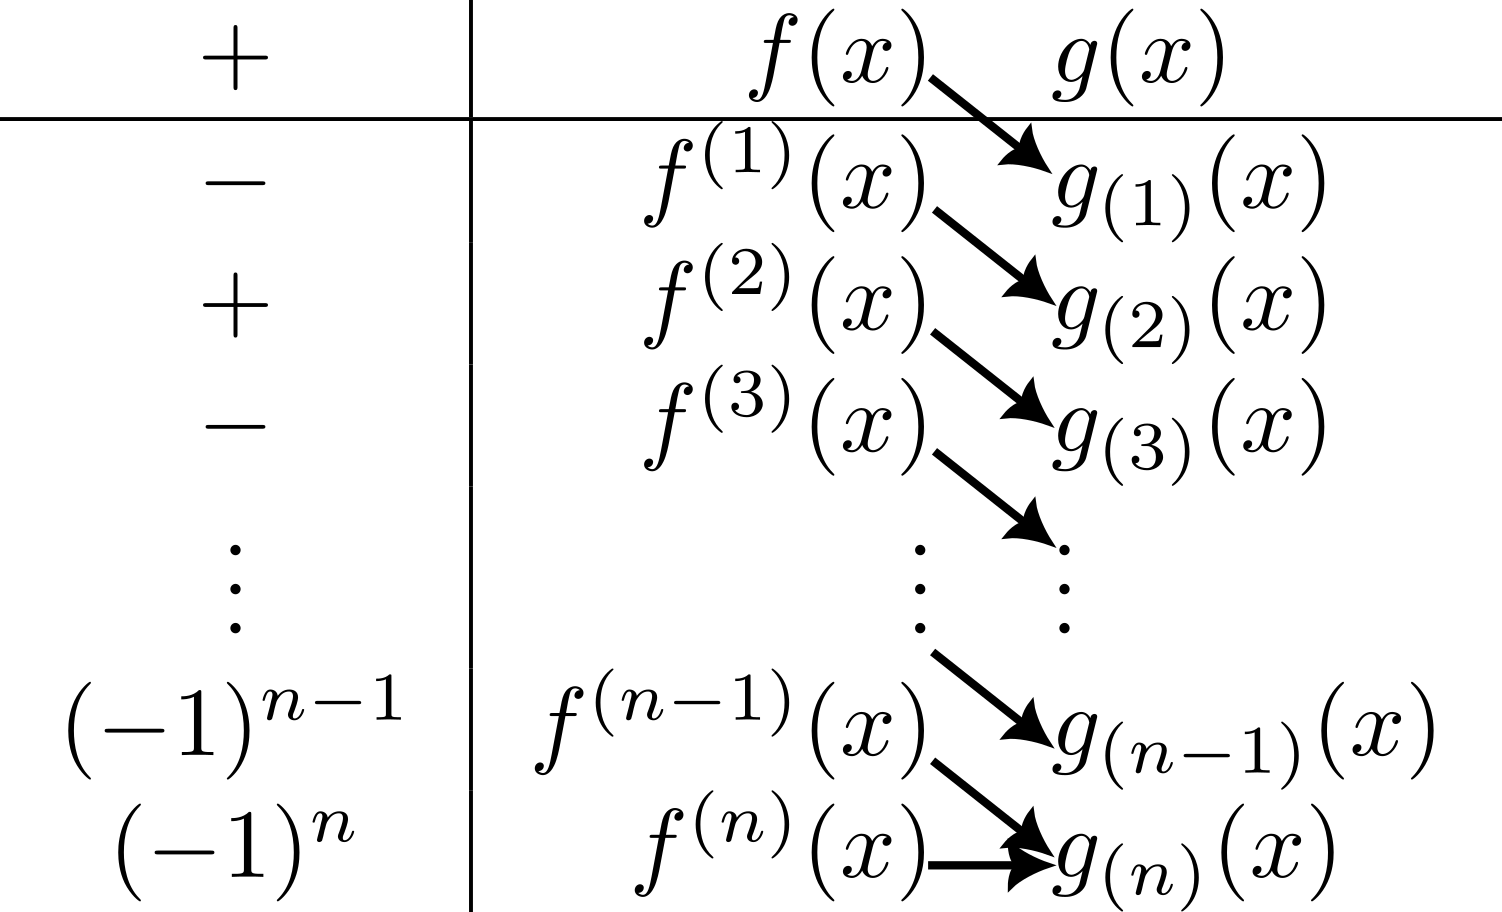
\includegraphics[width=0.34\linewidth]{include/tabular-boundary.png}
    \end{figure}
    At the end of this process, the original integral has become 
    % \begin{equation*}
    %     \begin{split}
    %         \intl u(x)v(x) dx &= (u(x)v_{(1)}(x)-u^{(1)}(x)v_{(2)}(x)+u^{(2)}(x)v_{(3)}(x) + \cdots + (-1)^{n-1} u^{(n-1)}(x))\biggr\rvert_\mathrm{a}^\mathrm{b}\\ &+ \intl v^{(4)}(x)u(x) dx.
    %     \end{split}
    % \end{equation*}
    \begin{equation*}
        \begin{split}
            \intl u(x)v(x) dx &= \left(\sum_{i=1}^{n} (-1)^{i-1}u^{(i-1)}(x)v_{(i)}(x)\right)\biggr\rvert_\mathrm{a}^\mathrm{b} + (-1)^n\intl u^{(n)}(x)v_{(n)}(x) dx.
        \end{split}
    \end{equation*}
\subsection{The Mean Value Theorem}
    The mean value theorem for integration states that for any function \(f\) which is integrable on \([a,b]\), there exists a value \(c\) where \(a < c < b\) such that
    \begin{equation*}
        \int_{a}^{b} f'(x)dx = f'(c)(b-a).
    \end{equation*}
\subsection{Big O Notation} \label{sec:BigO}
Big O notation is used to describe the limiting behavior of a function as the argument tends to some value or plus or minus infinity. By \(f(x)=O(g(x))\) as \(x\to x_0\) we mean that \(\frac{f(x)}{g(x)}\) is bounded as \(x\to x_0\). For example 
\begin{equation*}
    \sin 6x = O(1) \text{ as } x\to \inf.
\end{equation*}

\subsection{Alternative Method of Green's Functions}
In this text, we approach finding the Green's function by finding the adjoint operator and then defining 
\begin{equation*}
    \Lstar G = \d(\x-x).
\end{equation*}
Instead, one can find an alternative version of the Green's function, which we denote by \(G^*\), using the original differential operator acting on \(u\). 

Suppose a differential equation is given by
\begin{equation*}
    \L_x u = \phi.
\end{equation*}
We can define \(G^*(\xi,x)\) to be a function that satisfies,
\begin{equation*}
    \L_x G^* = \d(\x-x).
\end{equation*}
Consider
\begin{equation*}
    u(x) = \intl G^*(\x,x)\phi(\x)d\x.
\end{equation*}
Assuming \(G^*\) may be chosen so that the boundary conditions are satisfied,
\begin{equation*}
    \begin{split}
        \L_x u &= \L_x \intl G^*(\x,x)\phi(\x)d\x\\ 
        &= \intl \L_xG^*(\x,x)\phi(\x)d\x  \\ 
        &= \intl \d(\x-x)\phi(x)dx\\  
        &= \phi(x)
    \end{split}
\end{equation*}
so long as the equation \(\L_x\int = \int \L_x\) may be justified.


\addcontentsline{toc}{section}{References}

\bibliographystyle{alpha}
\bibliography{include/biblio}
Greenberg, Michael D. Applications of Green’s Functions in Science and Engineering. Dover

Publications, 2015.\\
Roach, G. F. Green’s Functions. Cambridge University Press, 1982.


\printindex

\end{document}
